% Options for packages loaded elsewhere
\PassOptionsToPackage{unicode}{hyperref}
\PassOptionsToPackage{hyphens}{url}
\PassOptionsToPackage{dvipsnames,svgnames,x11names}{xcolor}
%
\documentclass[
  letterpaper,
  DIV=11,
  numbers=noendperiod]{scrartcl}

\usepackage{amsmath,amssymb}
\usepackage{setspace}
\usepackage{iftex}
\ifPDFTeX
  \usepackage[T1]{fontenc}
  \usepackage[utf8]{inputenc}
  \usepackage{textcomp} % provide euro and other symbols
\else % if luatex or xetex
  \usepackage{unicode-math}
  \defaultfontfeatures{Scale=MatchLowercase}
  \defaultfontfeatures[\rmfamily]{Ligatures=TeX,Scale=1}
\fi
\usepackage{lmodern}
\ifPDFTeX\else  
    % xetex/luatex font selection
  \setmainfont[]{Times New Roman}
  \setmonofont[]{DejaVu Sans Mono}
\fi
% Use upquote if available, for straight quotes in verbatim environments
\IfFileExists{upquote.sty}{\usepackage{upquote}}{}
\IfFileExists{microtype.sty}{% use microtype if available
  \usepackage[]{microtype}
  \UseMicrotypeSet[protrusion]{basicmath} % disable protrusion for tt fonts
}{}
\usepackage{xcolor}
\setlength{\emergencystretch}{3em} % prevent overfull lines
\setcounter{secnumdepth}{5}
% Make \paragraph and \subparagraph free-standing
\ifx\paragraph\undefined\else
  \let\oldparagraph\paragraph
  \renewcommand{\paragraph}[1]{\oldparagraph{#1}\mbox{}}
\fi
\ifx\subparagraph\undefined\else
  \let\oldsubparagraph\subparagraph
  \renewcommand{\subparagraph}[1]{\oldsubparagraph{#1}\mbox{}}
\fi


\providecommand{\tightlist}{%
  \setlength{\itemsep}{0pt}\setlength{\parskip}{0pt}}\usepackage{longtable,booktabs,array}
\usepackage{calc} % for calculating minipage widths
% Correct order of tables after \paragraph or \subparagraph
\usepackage{etoolbox}
\makeatletter
\patchcmd\longtable{\par}{\if@noskipsec\mbox{}\fi\par}{}{}
\makeatother
% Allow footnotes in longtable head/foot
\IfFileExists{footnotehyper.sty}{\usepackage{footnotehyper}}{\usepackage{footnote}}
\makesavenoteenv{longtable}
\usepackage{graphicx}
\makeatletter
\def\maxwidth{\ifdim\Gin@nat@width>\linewidth\linewidth\else\Gin@nat@width\fi}
\def\maxheight{\ifdim\Gin@nat@height>\textheight\textheight\else\Gin@nat@height\fi}
\makeatother
% Scale images if necessary, so that they will not overflow the page
% margins by default, and it is still possible to overwrite the defaults
% using explicit options in \includegraphics[width, height, ...]{}
\setkeys{Gin}{width=\maxwidth,height=\maxheight,keepaspectratio}
% Set default figure placement to htbp
\makeatletter
\def\fps@figure{htbp}
\makeatother

\usepackage{fontspec}
\usepackage{multirow}
\usepackage{multicol}
\usepackage{colortbl}
\usepackage{hhline}
\newlength\Oldarrayrulewidth
\newlength\Oldtabcolsep
\usepackage{longtable}
\usepackage{array}
\usepackage{hyperref}
\usepackage{float}
\usepackage{wrapfig}
% \usepackage{hyperref}
% \hypersetup{
%     colorlinks,
%     linkcolor={blue!100!black},
%     citecolor={blue!100!black},
%     urlcolor={blue!100!black}
% }
% \usepackage{apacite}
% \usepackage[round]{natbib} 
% \usepackage{graphicx}
% \usepackage{float}
% \usepackage{caption}
% \usepackage[toc,page]{appendix}
% \usepackage{booktabs,caption}
% \usepackage[flushleft]{threeparttable}
% \usepackage{tabularx}
\usepackage{sfmath}
\usepackage{fontspec}
\usepackage[utf8]{inputenc}
\usepackage{siunitx}
\usepackage{amsfonts}
\usepackage{amsmath}
% \usepackage{xcolor}
% \usepackage{scrextend}
% \deffootnote[2em]{2em}{1em}{\textsuperscript{\thefootnotemark}\,}
% \newcolumntype{Y}{>{\centering\arraybackslash}X}
% \usepackage[a4paper]{geometry}
% \usepackage{caption}
% \usepackage[bottom,flushmargin,hang,multiple]{footmisc}
% \usepackage{pdflscape}
% \usepackage[paper=portrait,pagesize]{typearea}
% \usepackage{rotating}
% \usepackage{fullpage}
% \usepackage{tabu}
\usepackage{lscape}
\newcommand{\blandscape}{\begin{landscape}}
\newcommand{\elandscape}{\end{landscape}}
\usepackage{rotating}
\newcommand{\bsideways}{\begin{sidewaystable}[htbp]}
\newcommand{\esideways}{\end{sidewaystable}}
\KOMAoption{captions}{tableheading}
\makeatletter
\@ifpackageloaded{caption}{}{\usepackage{caption}}
\AtBeginDocument{%
\ifdefined\contentsname
  \renewcommand*\contentsname{Table of contents}
\else
  \newcommand\contentsname{Table of contents}
\fi
\ifdefined\listfigurename
  \renewcommand*\listfigurename{List of Figures}
\else
  \newcommand\listfigurename{List of Figures}
\fi
\ifdefined\listtablename
  \renewcommand*\listtablename{List of Tables}
\else
  \newcommand\listtablename{List of Tables}
\fi
\ifdefined\figurename
  \renewcommand*\figurename{Figure}
\else
  \newcommand\figurename{Figure}
\fi
\ifdefined\tablename
  \renewcommand*\tablename{Table}
\else
  \newcommand\tablename{Table}
\fi
}
\@ifpackageloaded{float}{}{\usepackage{float}}
\floatstyle{ruled}
\@ifundefined{c@chapter}{\newfloat{codelisting}{h}{lop}}{\newfloat{codelisting}{h}{lop}[chapter]}
\floatname{codelisting}{Listing}
\newcommand*\listoflistings{\listof{codelisting}{List of Listings}}
\makeatother
\makeatletter
\makeatother
\makeatletter
\@ifpackageloaded{caption}{}{\usepackage{caption}}
\@ifpackageloaded{subcaption}{}{\usepackage{subcaption}}
\makeatother
\ifLuaTeX
  \usepackage{selnolig}  % disable illegal ligatures
\fi
\usepackage[round]{natbib}
\bibliographystyle{apalike}
\usepackage{bookmark}

\IfFileExists{xurl.sty}{\usepackage{xurl}}{} % add URL line breaks if available
\urlstyle{same} % disable monospaced font for URLs
\hypersetup{
  colorlinks=true,
  linkcolor={blue!100!black},
  filecolor={Maroon},
  citecolor={blue!100!black},
  urlcolor={blue!100!black},
  pdfcreator={LaTeX via pandoc}}

\author{}
\date{}

\begin{document}

\title{ARM versus FRM in South Africa}

\author {Xolani Sibande\footnote{Economic Research Department, South African Reserve Bank; Email: xolani.sibande@resbank.co.za.} \and
Khutso Thobakgale\footnote{Economic Research Department, South African Reserve Bank; Email: khutso.thobekgale@resbank.co.za.}}


\date{\today}
\maketitle

\begin{abstract}
Ipsum

\end{abstract}

\noindent\textbf{Keywords}: \\
\textbf{JEL Codes}: 
\newpage

\setstretch{1.5}
\section{Introduction}\label{introduction}

\section{Literature Review}\label{literature-review}

A fixed rate mortgage can be referred to as a mortgage where the
borrower is guaranteed a fixed rate over the duration of the mortgage.
On the other hand, the adjustable-rate mortgage has an interest rate
that fluctuates over time based on the existing market rate.

Literature suggests that demand and supply factors drive the choice
between ARMs and FRMs. On the demand side borrowers financial condition
plays a significant role. \citet{baesel1980allocation} support this
statement with their analysis of the considerations borrowers make
between fixed versus index-linked mortgages. They found that borrower's
choice of mortgage depends on current the relationship between future
income and inflation.

\citet{statman1982fixed}, agrees with \citet{baesel1980allocation} that
borrower's preferences for fixed rate or index-linked mortgages depend
on the relationship between the rate of changes in income and the rate
of inflation. However, \citet{statman1982fixed} adds that borrowers
preferences also depend on the relationship between changes in the net
value of houses and the rate of inflation.

This is supported by the work of \citet{campbell2003household} who
derive relevant theoretical predictions by treating mortgage choice as a
problem in household risk management. In their framework, households
with low income and low levels of saving are likely to choose the loan
with the lowest interest rate. This tends to be an adjustable-rate
mortgage as a fixed rate mortgage often includes a term premium and the
cost of the prepayment option. \citet{campbell2003household} build on
this by arguing that the form of the mortgage contract can have
significant effects on household welfare and asked how a household
should make the choice between FRM and ARM. Their findings showed that
homeowners with smaller houses relative to income, more stable income,
lower risk aversion, more lenient treatment in bankruptcy, and a higher
probability of moving should find ARMs more attractive. A further
argument for ARMs is provided by \citet{cocco2013evidence} who states
that one the biggest advantages of an adjustable-rate mortgage is the
ability of borrowers to make limited payments in certain instances (when
resources are low), compensating in periods when their resources are
abundant \citep{cocco2013evidence}.

This heavy depends on homeowners being properly informed. Research by
\citet{paiella2007choosing} examined whether households can accurately
assess their circumstances in terms of (non-mortgage related) risk
exposure and make an appropriate choice of either a FRM or ARM. They
showed that household characteristics are irrelevant for the choice of
mortgage.

The choice between a fixed and adjustable mortgage was largely based on
whether households faced liquidity constraints. Households that face
liquidity constraints tend to favour ARMs because they have lower
initial payments. These households tend to overlook the overall cost of
the mortgage and \citet{paiella2007choosing} argue that they do not
fully consider the risk of a rise in the reference interest rate.
Lenders on the other hand price the risk too high and borrowers end up
paying a higher price for the benefit of the lower initial payments.

\citet{campbell2006household} use the American Housing Survey to show
evidence that mortgage borrowers make several mistakes that leads to
important implications for equilibrium in the mortgage market. For
example, he finds that the decision to refinance FRM is challenging for
many households, particularly poorer and less educated ones, and
therefore they pay higher mortgage rates than necessary.

\citet{kim2016borrower} expand on this with their research paper
documenting the relationship between the perceived borrower's risk and
the choice between undertaking an adjustable or a fixed rate mortgage.
They discover that during high (low) short-term interest rate
environments, borrowers perceive a low (high) probability of rate
increases (decreases). This explained their desire for ARMs over FRMs.
Hence, the desire for ARMs (FRMs). However, they found that during a
down housing market borrowers tended to avoid ARMs due to an increased
perceived risk.

However, a disadvantage of an ARM is that it exposes borrowers to the
income risk of short-term variability in the periodic payments resulting
in households who cannot afford to take this risk (for example in case
of high loan-to-income ratio and low financial wealth) opting for an FRM
instead. These findings are validated by empirical papers by
\citep{paiella2007choosing, fornero2011effect, ehrmann2017mortgage}

Another factor that plays a key role in mortgage choice is the financial
literacy of borrowers
\citep{gathergood2017financial, fornero2011effect, agarwal2012adverse}.
Findings suggest that more educated borrowers understand that FRMs are
more expensive than ARMs due to the term premium and the cost of the
prepayment option. They are also aware of the potential risks that come
with ARMs \citep{fornero2011effect}.

On the supply side, factors such as bank funding and liquidity
constraints determine the type of loan offered. Research by
\citet{fuster2015securitization}, and \citet{basten2017banks} shows it
is the lower bank bond spreads, lower deposit pass-through, lower
exposure to interest rate risk and higher access to securitization make
that made banks more prone to offer fixed rate loans.

Offering flexible rate mortgages for banks has been shown to have a
positive impact on a banks uptake of mortgages. An example of this is
given by \citet{cocco2013evidence} who utilized a specialized mortgage
program marketed by a U.S bank to certain borrowers during 2004 and
2005. The bank in the study offered different versions of option
adjustable-rate mortgages that allowed for negative amortization.
\citet{cocco2013evidence} found that offering the program led to a more
than 35 percent increase in the bank's mortgage originations volume.

This is due to the bank in the study offering different versions of
option adjusted rate mortgages that allowed for negative amortization.
This offered significant flexibility to borrowers leading to their
popularity during the housing boom form 2006. An increase by 12 to 40
percent was observed in some well performing markets
\citep{piskorski2010optimal, krainer2014mortgage}.

Offering flexibility comes with significant loan performance costs for
the bank, though this is not immediately apparent from a casual analysis
\citep{cocco2013evidence}. Flexible loans exhibit lower delinquency
risks, controlling for observable borrower and transaction
characteristics. This result, however, may be driven by unobserved
borrower characteristics.

Finally, there are other macroeconomic factors such as current and
future expected interest rates as well as the unemployment rate and the
macroeconomic history of a country that influence mortgage choice.

\subsection{Monetary policy
transmission}\label{monetary-policy-transmission}

According to \citet{mishkin2007housing} monetary policy affects the
housing market directly or indirectly through the following channels.
Direct effects can be user cost of capital, expectations of future
house-price movements, and housing supply. Indirect effects are the
standard wealth effects from housing prices, balance sheet,
credit-channel effects on consumer spending, and balance sheet,
credit-channel effects on housing demand.

Through these channels the increase or decrease in the policy rate can
impact mortgages with flexible more than those with fixed rates. This is
evidenced by \citet{garriga2017mortgages} who found that the
transmission mechanism is stronger under adjustable- than fixed-rate
mortgages. They found that the real effects of the nominal shock turned
out to be stronger under an ARM than an FRM
\citep{garriga2017mortgages}.

\subsection{Interest rate passthrough}\label{interest-rate-passthrough}

Some of the factors that affect homeowners average interest rate on
fixed rate mortgages include refinancing, entry channel and exit
channel. Refinancing of fixed-rate mortgages to mortgages with lower
interest rates have contributed to a significant part of the decrease in
homeowners' average interest rate since the financial crisis. The entry
channel comprises borrowers who raise new fixed-rate debt at the market
rate. New lending occurs in connection with relocations, switching from
other loan types and borrowers who for the first time enter the housing
market. The exit channel comprises borrowers with existing fixed-rate
mortgages who repay the debt by instalments or terminate their loans
without refinancing. Terminations typically cover relocations, switching
to other loan types and foreclosure auctions.

\section{Experiences from the rest of the
world}\label{experiences-from-the-rest-of-the-world}

In contrast to South Africa and many countries, in the United States
80\% of mortgages have fixed rates. \citet{botsch2023long} link this to
the long-lasting effects of the Great Depression. This points to
personal experiences with interest rates having an impact on interest
rate expectations and mortgage choices. \citet{botsch2023long} link this
to the long-lasting effects of the Great Inflation. Personal experiences
with interest rates affect interest rate expectations and mortgage
choices. This is consistent with the idea that historically high
inflation rates can predict the prevalence of fixed mortgages
internationally. Despite the recent domination of fixed interest rates
in the US, before the 1930s variable rates were the dominant type of
mortgage. It was due to the Great depression that many borrowers
defaulted on their payments. Following these policies to purchase
long-term rate mortgages from banks so that lenders can shed the
interest rate risk associated with holding these assets to maturity
resulting in the dominance of FRM for the next 40 years.

\subsection{Australia}\label{australia}

Australia's mortgage market differs from the United States and other
countries in the sense that the mortgage market transactions are not
influenced by institutional structures such as Fannie Mac and Freddie
Mac in the USA, government mortgage insurance as seen in the Netherlands
and government security guarantees in Japan and Canada
\citep{campbell2006household, frame2005fussing}.
\citet{dungey2015mortgage} state that securitization in Australia plays
a minimal role in securing funds for major banks. They also mention that
there is strong prudential regulation, but no public mortgage insurance
scheme and that no government deposit guarantee existed prior to the
impact of the financial crisis in 2008-2009.

Like South Africa, Australia's mortgage is dominated by ARMs. But
Australia's market is characterized by a credit frontier loan written
for terms up to 30 years, with the interest rate adjustable with the
discretion of the bank. In Australia borrowers consider the initial
interest rate and implicitly the loan amount they can access when
choosing a mortgage product \citet{dungey2018endogeneity}.
\citet{dungey2018endogeneity} show that the role of borrower
characteristics is insignificant in determining mortgage choice directly
and indirectly, through loan size and interest rate determination. In
short, \citet{dungey2018endogeneity} finding reveal the potential
effects of monetary policy transmission coupled with macro- and
micro-prudential regulation. They show that borrowers' mortgage risk
choices are mainly determined by mortgage prices and mortgage terms --
such as loan size, market conditions and borrower characteristics.

\subsection{Italy}\label{italy}

In Italy both demand and supply factors explain mortgage choice. On the
demand side, a reduction in interest rates leads to an increase in the
number of households holding a mortgage. On the supply side, the authors
claim there is a positive corelation between the number of bank branches
in a province and mortgages. Thus, there is significant probability that
inhabitants will hold a mortgage due to bank diffusion and competition.
Their results show evidence consistent with the hypothesis that ARMs are
more attractive for households that are currently facing a liquidity
constraint.

Additionally, they show that one of the most important factors that
influence their preference for ARMs is the high value they attribute to
the level of the initial payment. (Lower than FRM). On the lenders side,
they price the risk of high interest rates expensively leading to
borrowers paying a high price for the benefit of low initial payments.
Thus, banks tend to take less risk when offering rates while borrowers
don't fully consider the risk of the rise in the interest rate.

\subsection{Denmark}\label{denmark}

Denmark's mortgage environment consists of at least half of the
mortgages taken on fixed rates thus fixed rate mortgages constitute a
large proportion of the Danes' debt (Denmark's national bank). The
result of this is that in theory an interest rate decrease will only
result in lower current financing costs for homeowners with fixed-rate
mortgages if they prepay their existing loans and raise new loans with
lower rates.

Fixed rates in Denmark can be refinanced without the outstanding debt
being significantly increased making refinancing attractive when
interest rates decrease. The refinancing to lower interest rates has
boosted the impact on how quickly a change in interest rates has passed
to homeowners' mortgage rates. This has been particularly evident during
waves of refinancing. Approximately means that it takes five years for a
1 percent interest rate change to have a pass-through of 90 per cent,
while it takes 6.2 years for an interest rate change to have a
pass-through of 95 per cent for periods after major market rate
decreases. Refinancing of fixed-rate mortgages has thus supported the
transmission of monetary policy rates to homeowners' budgets making
policy rates particularly effective regardless of the mortgages not
being ARMs like in South Africa.

On reason for this is that Danish fixed rate mortgages are special
because borrowers can always redeem the loan at price 100 and thus
refinance the loan without incurring a significant increase in the
outstanding debt. Homeowners are thus protected from ending up with debt
that is expensive to repurchase in connection with interest rate
decreases. Providing a major reason why the Danish choose to finance
their mortgages with fixed rates.

\subsection{Euro Area}\label{euro-area}

In the euro area, fixed rate mortgages (FRMs) are dominant in Belgium,
France, Germany and the Netherlands. While adjustable-rate mortgages
(ARMs) are prevailing in Austria, Greece, Italy, Portugal, and Spain. A
study 12 countries claims that demand factors explain much of the total
variation in the share of FRMs. A smaller portion, below 19\% were
associated with bank supply factors. The remaining 9\% wasn't able to be
explained. In the 12 countries studied the demand side of the ARMs was
found to be positively influenced by the following factors. Firstly, a
historically high inflation volatility, and secondly a relatively high
degree of economic and financial literacy. Thirdly, the absence of
regulations to facilitate the use of such loans as collateral for bank
funding instruments, such as covered bonds and MBS, and lastly a marked
negative correlation between the unemployment rate and short-term
interest rates.

When it comes to FRMs the \citet{albertazzi2019fixed} concludes that at
least part of the heterogeneity in the share of fixed rate mortgages
across economies seems to reflect an optimal allocation of interest rate
risk, given the differences in their business cycles and the
expectations that monetary policy will operate in a way that stabilizes
disposable income after housing costs were considered. Additionally, the
variation in the share of FRMs to total new mortgages differs across
countries as well, with little variation over time in Germany and
Portugal, but far more in Italy and Greece \citep{albertazzi2019fixed}.
This suggest that there is monetary policy transmission heterogeneity
across countries.

\newpage

\bsideways

\global\setlength{\Oldarrayrulewidth}{\arrayrulewidth}

\global\setlength{\Oldtabcolsep}{\tabcolsep}

\setlength{\tabcolsep}{0pt}

\renewcommand*{\arraystretch}{0.5}



\providecommand{\ascline}[3]{\noalign{\global\arrayrulewidth #1}\arrayrulecolor[HTML]{#2}\cline{#3}}

\begin{longtable}[l]{|p{0.66in}|p{0.10in}|p{8.03in}}

\caption{\label{tbl-summary}Summary of the international experience}

\tabularnewline

\ascline{0.75pt}{000000}{1-3}

\multicolumn{1}{!{\color[HTML]{FFFFFF}\vrule width 1pt}>{\centering}m{\dimexpr 0.66in+0\tabcolsep}}{\textcolor[HTML]{000000}{\fontsize{7}{14}\selectfont{\global\setmainfont{Times New Roman}{Country}}}} & \multicolumn{1}{!{\color[HTML]{FFFFFF}\vrule width 1pt}>{\centering}m{\dimexpr 0.1in+0\tabcolsep}}{\textcolor[HTML]{000000}{\fontsize{7}{14}\selectfont{\global\setmainfont{Times New Roman}{Mortgage}}}} & \multicolumn{1}{!{\color[HTML]{FFFFFF}\vrule width 1pt}>{\centering}m{\dimexpr 8.03in+0\tabcolsep}!{\color[HTML]{FFFFFF}\vrule width 1pt}}{\textcolor[HTML]{000000}{\fontsize{7}{14}\selectfont{\global\setmainfont{Times New Roman}{Reason\ for\ choice}}}} \\

\ascline{0.75pt}{000000}{1-3}\endfirsthead 

\ascline{0.75pt}{000000}{1-3}

\multicolumn{1}{!{\color[HTML]{FFFFFF}\vrule width 1pt}>{\centering}m{\dimexpr 0.66in+0\tabcolsep}}{\textcolor[HTML]{000000}{\fontsize{7}{14}\selectfont{\global\setmainfont{Times New Roman}{Country}}}} & \multicolumn{1}{!{\color[HTML]{FFFFFF}\vrule width 1pt}>{\centering}m{\dimexpr 0.1in+0\tabcolsep}}{\textcolor[HTML]{000000}{\fontsize{7}{14}\selectfont{\global\setmainfont{Times New Roman}{Mortgage}}}} & \multicolumn{1}{!{\color[HTML]{FFFFFF}\vrule width 1pt}>{\centering}m{\dimexpr 8.03in+0\tabcolsep}!{\color[HTML]{FFFFFF}\vrule width 1pt}}{\textcolor[HTML]{000000}{\fontsize{7}{14}\selectfont{\global\setmainfont{Times New Roman}{Reason\ for\ choice}}}} \\

\ascline{0.75pt}{000000}{1-3}\endhead



\multicolumn{1}{!{\color[HTML]{FFFFFF}\vrule width 1pt}>{\centering}m{\dimexpr 0.66in+0\tabcolsep}}{\textcolor[HTML]{000000}{\fontsize{7}{14}\selectfont{\global\setmainfont{Times New Roman}{USA}}}} & \multicolumn{1}{!{\color[HTML]{FFFFFF}\vrule width 1pt}>{\centering}m{\dimexpr 0.1in+0\tabcolsep}}{\textcolor[HTML]{000000}{\fontsize{7}{14}\selectfont{\global\setmainfont{Times New Roman}{FRMs}}}} & \multicolumn{1}{!{\color[HTML]{FFFFFF}\vrule width 1pt}>{\centering}m{\dimexpr 8.03in+0\tabcolsep}!{\color[HTML]{FFFFFF}\vrule width 1pt}}{\textcolor[HTML]{000000}{\fontsize{7}{14}\selectfont{\global\setmainfont{Times New Roman}{The\ prevalence\ of\ FRM\ can\ be\ explained\ by\ the\ lasting\ effects\ of\ the\ great\ inflation.\ Experience\ of\ high\ interest\ rates\ affected\ interest\ rate\ expectations\ and\ mortgage\ choices\ (Botsch\ and\ Malmendier,\ 2023)}}}} \\

\ascline{1pt}{FFFFFF}{1-3}



\multicolumn{1}{!{\color[HTML]{FFFFFF}\vrule width 1pt}>{\centering}m{\dimexpr 0.66in+0\tabcolsep}}{\textcolor[HTML]{000000}{\fontsize{7}{14}\selectfont{\global\setmainfont{Times New Roman}{Italy}}}} & \multicolumn{1}{!{\color[HTML]{FFFFFF}\vrule width 1pt}>{\centering}m{\dimexpr 0.1in+0\tabcolsep}}{\textcolor[HTML]{000000}{\fontsize{7}{14}\selectfont{\global\setmainfont{Times New Roman}{Both}}}} & \multicolumn{1}{!{\color[HTML]{FFFFFF}\vrule width 1pt}>{\centering}m{\dimexpr 8.03in+0\tabcolsep}!{\color[HTML]{FFFFFF}\vrule width 1pt}}{\textcolor[HTML]{000000}{\fontsize{7}{14}\selectfont{\global\setmainfont{Times New Roman}{The\ choice\ mostly\ depends\ on\ the\ price\ of\ the\ mortgage\ and\ the\ liquidity\ of\ the\ household.}}}} \\

\ascline{1pt}{FFFFFF}{1-3}



\multicolumn{1}{!{\color[HTML]{FFFFFF}\vrule width 1pt}>{\centering}m{\dimexpr 0.66in+0\tabcolsep}}{\textcolor[HTML]{000000}{\fontsize{7}{14}\selectfont{\global\setmainfont{Times New Roman}{Germany}}}} & \multicolumn{1}{!{\color[HTML]{FFFFFF}\vrule width 1pt}>{\centering}m{\dimexpr 0.1in+0\tabcolsep}}{\textcolor[HTML]{000000}{\fontsize{7}{14}\selectfont{\global\setmainfont{Times New Roman}{FRM}}}} & \multicolumn{1}{!{\color[HTML]{FFFFFF}\vrule width 1pt}>{\centering}m{\dimexpr 8.03in+0\tabcolsep}!{\color[HTML]{FFFFFF}\vrule width 1pt}}{\textcolor[HTML]{000000}{\fontsize{7}{14}\selectfont{\global\setmainfont{Times New Roman}{The\ sophisticated\ rental\ market\ enables\ households\ to\ save\ their\ own\ funds\ for\ house\ purchases\ (Voigtlander,\ 2014)}}}} \\

\ascline{1pt}{FFFFFF}{1-3}



\multicolumn{1}{!{\color[HTML]{FFFFFF}\vrule width 1pt}>{\centering}m{\dimexpr 0.66in+0\tabcolsep}}{\textcolor[HTML]{000000}{\fontsize{7}{14}\selectfont{\global\setmainfont{Times New Roman}{Spain}}}} & \multicolumn{1}{!{\color[HTML]{FFFFFF}\vrule width 1pt}>{\centering}m{\dimexpr 0.1in+0\tabcolsep}}{\textcolor[HTML]{000000}{\fontsize{7}{14}\selectfont{\global\setmainfont{Times New Roman}{ARM\ with\ recent\ surge\ of\ FRM}}}} & \multicolumn{1}{!{\color[HTML]{FFFFFF}\vrule width 1pt}>{\centering}m{\dimexpr 8.03in+0\tabcolsep}!{\color[HTML]{FFFFFF}\vrule width 1pt}}{\textcolor[HTML]{000000}{\fontsize{7}{14}\selectfont{\global\setmainfont{Times New Roman}{Since\ the\ 90’s\ ARM\ was\ preferred\ until\ contracts\ included\ upwards\ and\ downward\ limits\ leading\ to\ an\ increase\ in\ FRM\ (Gomez-pomar,\ Segura-Moreiras\ and\ Spruk,\ 2021)}}}} \\

\ascline{1pt}{FFFFFF}{1-3}



\multicolumn{1}{!{\color[HTML]{FFFFFF}\vrule width 1pt}>{\centering}m{\dimexpr 0.66in+0\tabcolsep}}{\textcolor[HTML]{000000}{\fontsize{7}{14}\selectfont{\global\setmainfont{Times New Roman}{United\ Kingdom}}}} & \multicolumn{1}{!{\color[HTML]{FFFFFF}\vrule width 1pt}>{\centering}m{\dimexpr 0.1in+0\tabcolsep}}{\textcolor[HTML]{000000}{\fontsize{7}{14}\selectfont{\global\setmainfont{Times New Roman}{FRM}}}} & \multicolumn{1}{!{\color[HTML]{FFFFFF}\vrule width 1pt}>{\centering}m{\dimexpr 8.03in+0\tabcolsep}!{\color[HTML]{FFFFFF}\vrule width 1pt}}{\textcolor[HTML]{000000}{\fontsize{7}{14}\selectfont{\global\setmainfont{Times New Roman}{Long\ term\ fixed\ mortgage\ rates\ have\ become\ cheaper\ than\ other\ alternatives\ since\ 2016.\ The\ cheaper\ borrowing\ cost\ is\ seen\ as\ a\ reason\ for\ the\ increase\ in\ fixed\ rate\ mortgages.\ (Bank\ of\ England,\ 2024)}}}} \\

\ascline{1pt}{FFFFFF}{1-3}



\multicolumn{1}{!{\color[HTML]{FFFFFF}\vrule width 1pt}>{\centering}m{\dimexpr 0.66in+0\tabcolsep}}{\textcolor[HTML]{000000}{\fontsize{7}{14}\selectfont{\global\setmainfont{Times New Roman}{France}}}} & \multicolumn{1}{!{\color[HTML]{FFFFFF}\vrule width 1pt}>{\centering}m{\dimexpr 0.1in+0\tabcolsep}}{\textcolor[HTML]{000000}{\fontsize{7}{14}\selectfont{\global\setmainfont{Times New Roman}{FRM}}}} & \multicolumn{1}{!{\color[HTML]{FFFFFF}\vrule width 1pt}>{\centering}m{\dimexpr 8.03in+0\tabcolsep}!{\color[HTML]{FFFFFF}\vrule width 1pt}}{\textcolor[HTML]{000000}{\fontsize{7}{14}\selectfont{\global\setmainfont{Times New Roman}{There\ is\ little\ rate\ differential\ between\ ARM\ and\ FRM\ due\ to\ the\ low\ interest\ rate\ environment\ resulting\ in\ little\ incentive\ to\ take\ on\ an\ ARM\ (Kish,\ 2022)}}}} \\

\ascline{0.75pt}{000000}{1-3}


\end{longtable}

\arrayrulecolor[HTML]{000000}

\global\setlength{\arrayrulewidth}{\Oldarrayrulewidth}

\global\setlength{\tabcolsep}{\Oldtabcolsep}

\renewcommand*{\arraystretch}{1}

\esideways
\newpage

\section{The South African mortgage
market}\label{the-south-african-mortgage-market}

Housing finance in South Africa is largely determined by two factors,
which include cost of funding and the lending risk in the different
markets \citep{kajimo2006role}. Factors such as country risk, interest
rate, inflation rate and rental price are some of the major variables
that influence the housing market \citep{habanabakize2022political}.
However, \citet{kajimo2006role} points out that low-income groups are
held back because they cannot get access to formal finance for them to
build or improve houses or supplement housing subsidies to get bigger
houses \citep{kajimo2006role}. This is an unfortunate characteristic of
the housing market in South Africa that differentiates it form other
more advanced economies. Additionally, most of the low-income households
in South Africa are dependent on the government for house subsidies.

One of the causes from the supply side is the reluctance of banks Banks
to operate in the low-income group housing market, and this
unwillingness causes a shortage problem in the country
\citep{kajimo2006role}. The result is that high and middle-income groups
are provided for, the banks, especially the larger banks have little
engagement with the low-income groups \citep{kajimo2006role}. The impact
of inflation was found to be mostly insignificant on the proportion of
mortgages advanced to low-, middle- and high-income households in rand
value but was found to be significant and negative for the proportion of
mortgages advanced to middle- income households in volume. This finding
is particularly important to monetary policy transmission as the South
African Reserve Bank must consider the impact that inflation has on the
volume of mortgages rather than the rand value.

With this analysis of the south African mortgage in mind, there is a
clear separation between low-income and middle-to-higher income groups
further complicating the analysis of the housing market. Additionally,
there is limited data showing which income group prefers what type of
mortgage placing a limitation on this study. Regardless there are
certain observations we can make with the data we have. This is explored
in the following section of this study. First, we will go through some
of the characteristics of the mortgage markets in certain countries
around the world to see if there are any similarities or differences
that can help understand not only South Africa's mortgage market but the
housing market in general.

\section{The prevalence of ARMs in South
Africa}\label{the-prevalence-of-arms-in-south-africa}

\textbf{?@fig-harm} and \textbf{?@fig-carm} display the dominance of
ARMs over FRMs in South Africa's mortgage market. For household
mortgages the share of total mortgages consistently been above 90\% from
2008 to 2023. On the other hand, from 2008 to 2023, ARMs have been at
least 80\% on average for corporations. From 2008 to around late 2010
flexible mortgages were above 90\%, this was followed by a decline from
2010 to 2013. One explanation for this could be the 2008/2009 financial
crisis. This is consistent with findings from \citet{kim2016borrower}
who state that during a down housing market borrowers tended to avoid
ARMs due to an increased perceived risk. From 2013 onwards the rates
remained stable around 80\% until 2020 where there was an external shock
in the form of Covid 19 global pandemic.

Thereafter we see the rates go back to just above 80\% of the share of
mortgages. But what explains the portion of fixed rate mortgages?
\citet{damen2016effect} state that this is due to households' (typically
high earning) households preference to spend a fixed fraction of their
income on housing. This assists households budget their largest expense
(housing) allowing for them to spend the remainder on other expenses
(food, cars etc).

There are two instances on the graph (2009 and late 2022) where the ARMs
intersect with the FRMs. Lending rates, similarly, to deposit rates,
follow the movements in the repo rate. During the COVID-19 pandemic, the
weighted average lending rate has been reflecting a noticeable increase
in the risk profile of borrowers following the national lockdown from
March 2020, along with a visible difference between the rates for
households and companies.

\section{Data and methodology}\label{data-and-methodology}

\section{Results}\label{results}

\section{Conclusion}\label{conclusion}

\newpage

\section*{References}\label{references}
\addcontentsline{toc}{section}{References}

\renewcommand{\bibsection}{}
\bibliography{references.bib}

\setcounter{section}{0}
\renewcommand{\thesection}{\Alph{section}}

\setcounter{table}{0}
\renewcommand{\thetable}{A\arabic{table}}

\setcounter{figure}{0}
\renewcommand{\thefigure}{A\arabic{figure}}

\newpage

\section{Appendix}\label{appendix}

\subsection{Bank selection}\label{bank-selection}

\global\setlength{\Oldarrayrulewidth}{\arrayrulewidth}

\global\setlength{\Oldtabcolsep}{\tabcolsep}

\setlength{\tabcolsep}{0pt}

\renewcommand*{\arraystretch}{0.4}



\providecommand{\ascline}[3]{\noalign{\global\arrayrulewidth #1}\arrayrulecolor[HTML]{#2}\cline{#3}}

\begin{longtable}[l]{|p{1.28in}|p{0.65in}|p{1.10in}|p{0.94in}|p{0.96in}|p{1.13in}|p{0.72in}}

\caption{\label{tbl-bank_selection}Bank selection}

\tabularnewline

\ascline{0.75pt}{000000}{1-7}

\multicolumn{1}{!{\color[HTML]{FFFFFF}\vrule width 1pt}>{\raggedright}m{\dimexpr 1.28in+0\tabcolsep}}{\textcolor[HTML]{000000}{\fontsize{7}{14}\selectfont{\global\setmainfont{Times New Roman}{Banks}}}} & \multicolumn{1}{!{\color[HTML]{FFFFFF}\vrule width 1pt}>{\raggedright}m{\dimexpr 0.65in+0\tabcolsep}}{\textcolor[HTML]{000000}{\fontsize{7}{14}\selectfont{\global\setmainfont{Times New Roman}{n}}}} & \multicolumn{1}{!{\color[HTML]{FFFFFF}\vrule width 1pt}>{\raggedright}m{\dimexpr 1.1in+0\tabcolsep}}{\textcolor[HTML]{000000}{\fontsize{7}{14}\selectfont{\global\setmainfont{Times New Roman}{missing\_values}}}} & \multicolumn{1}{!{\color[HTML]{FFFFFF}\vrule width 1pt}>{\raggedright}m{\dimexpr 0.94in+0\tabcolsep}}{\textcolor[HTML]{000000}{\fontsize{7}{14}\selectfont{\global\setmainfont{Times New Roman}{nan\_values}}}} & \multicolumn{1}{!{\color[HTML]{FFFFFF}\vrule width 1pt}>{\raggedright}m{\dimexpr 0.96in+0\tabcolsep}}{\textcolor[HTML]{000000}{\fontsize{7}{14}\selectfont{\global\setmainfont{Times New Roman}{zero\_values}}}} & \multicolumn{1}{!{\color[HTML]{FFFFFF}\vrule width 1pt}>{\raggedright}m{\dimexpr 1.13in+0\tabcolsep}}{\textcolor[HTML]{000000}{\fontsize{7}{14}\selectfont{\global\setmainfont{Times New Roman}{negative\_values}}}} & \multicolumn{1}{!{\color[HTML]{FFFFFF}\vrule width 1pt}>{\raggedright}m{\dimexpr 0.72in+0\tabcolsep}!{\color[HTML]{FFFFFF}\vrule width 1pt}}{\textcolor[HTML]{000000}{\fontsize{7}{14}\selectfont{\global\setmainfont{Times New Roman}{recon}}}} \\

\ascline{0.75pt}{000000}{1-7}\endfirsthead 

\ascline{0.75pt}{000000}{1-7}

\multicolumn{1}{!{\color[HTML]{FFFFFF}\vrule width 1pt}>{\raggedright}m{\dimexpr 1.28in+0\tabcolsep}}{\textcolor[HTML]{000000}{\fontsize{7}{14}\selectfont{\global\setmainfont{Times New Roman}{Banks}}}} & \multicolumn{1}{!{\color[HTML]{FFFFFF}\vrule width 1pt}>{\raggedright}m{\dimexpr 0.65in+0\tabcolsep}}{\textcolor[HTML]{000000}{\fontsize{7}{14}\selectfont{\global\setmainfont{Times New Roman}{n}}}} & \multicolumn{1}{!{\color[HTML]{FFFFFF}\vrule width 1pt}>{\raggedright}m{\dimexpr 1.1in+0\tabcolsep}}{\textcolor[HTML]{000000}{\fontsize{7}{14}\selectfont{\global\setmainfont{Times New Roman}{missing\_values}}}} & \multicolumn{1}{!{\color[HTML]{FFFFFF}\vrule width 1pt}>{\raggedright}m{\dimexpr 0.94in+0\tabcolsep}}{\textcolor[HTML]{000000}{\fontsize{7}{14}\selectfont{\global\setmainfont{Times New Roman}{nan\_values}}}} & \multicolumn{1}{!{\color[HTML]{FFFFFF}\vrule width 1pt}>{\raggedright}m{\dimexpr 0.96in+0\tabcolsep}}{\textcolor[HTML]{000000}{\fontsize{7}{14}\selectfont{\global\setmainfont{Times New Roman}{zero\_values}}}} & \multicolumn{1}{!{\color[HTML]{FFFFFF}\vrule width 1pt}>{\raggedright}m{\dimexpr 1.13in+0\tabcolsep}}{\textcolor[HTML]{000000}{\fontsize{7}{14}\selectfont{\global\setmainfont{Times New Roman}{negative\_values}}}} & \multicolumn{1}{!{\color[HTML]{FFFFFF}\vrule width 1pt}>{\raggedright}m{\dimexpr 0.72in+0\tabcolsep}!{\color[HTML]{FFFFFF}\vrule width 1pt}}{\textcolor[HTML]{000000}{\fontsize{7}{14}\selectfont{\global\setmainfont{Times New Roman}{recon}}}} \\

\ascline{0.75pt}{000000}{1-7}\endhead



\multicolumn{1}{!{\color[HTML]{FFFFFF}\vrule width 1pt}>{\raggedright}m{\dimexpr 1.28in+0\tabcolsep}}{\textcolor[HTML]{000000}{\fontsize{7}{14}\selectfont{\global\setmainfont{Times New Roman}{Total\ Banks}}}} & \multicolumn{1}{!{\color[HTML]{FFFFFF}\vrule width 1pt}>{\raggedright}m{\dimexpr 0.65in+0\tabcolsep}}{\textcolor[HTML]{000000}{\fontsize{7}{14}\selectfont{\global\setmainfont{Times New Roman}{768}}}} & \multicolumn{1}{!{\color[HTML]{FFFFFF}\vrule width 1pt}>{\raggedright}m{\dimexpr 1.1in+0\tabcolsep}}{\textcolor[HTML]{000000}{\fontsize{7}{14}\selectfont{\global\setmainfont{Times New Roman}{0}}}} & \multicolumn{1}{!{\color[HTML]{FFFFFF}\vrule width 1pt}>{\raggedright}m{\dimexpr 0.94in+0\tabcolsep}}{\textcolor[HTML]{000000}{\fontsize{7}{14}\selectfont{\global\setmainfont{Times New Roman}{0}}}} & \multicolumn{1}{!{\color[HTML]{FFFFFF}\vrule width 1pt}>{\raggedright}m{\dimexpr 0.96in+0\tabcolsep}}{\textcolor[HTML]{000000}{\fontsize{7}{14}\selectfont{\global\setmainfont{Times New Roman}{0}}}} & \multicolumn{1}{!{\color[HTML]{FFFFFF}\vrule width 1pt}>{\raggedright}m{\dimexpr 1.13in+0\tabcolsep}}{\textcolor[HTML]{000000}{\fontsize{7}{14}\selectfont{\global\setmainfont{Times New Roman}{0}}}} & \multicolumn{1}{!{\color[HTML]{FFFFFF}\vrule width 1pt}>{\raggedright}m{\dimexpr 0.72in+0\tabcolsep}!{\color[HTML]{FFFFFF}\vrule width 1pt}}{\textcolor[HTML]{000000}{\fontsize{7}{14}\selectfont{\global\setmainfont{Times New Roman}{1.0}}}} \\

\ascline{1pt}{FFFFFF}{1-7}



\multicolumn{1}{!{\color[HTML]{FFFFFF}\vrule width 1pt}>{\raggedright}m{\dimexpr 1.28in+0\tabcolsep}}{\textcolor[HTML]{000000}{\fontsize{7}{14}\selectfont{\global\setmainfont{Times New Roman}{Standard\_Bank}}}} & \multicolumn{1}{!{\color[HTML]{FFFFFF}\vrule width 1pt}>{\raggedright}m{\dimexpr 0.65in+0\tabcolsep}}{\textcolor[HTML]{000000}{\fontsize{7}{14}\selectfont{\global\setmainfont{Times New Roman}{768}}}} & \multicolumn{1}{!{\color[HTML]{FFFFFF}\vrule width 1pt}>{\raggedright}m{\dimexpr 1.1in+0\tabcolsep}}{\textcolor[HTML]{000000}{\fontsize{7}{14}\selectfont{\global\setmainfont{Times New Roman}{0}}}} & \multicolumn{1}{!{\color[HTML]{FFFFFF}\vrule width 1pt}>{\raggedright}m{\dimexpr 0.94in+0\tabcolsep}}{\textcolor[HTML]{000000}{\fontsize{7}{14}\selectfont{\global\setmainfont{Times New Roman}{0}}}} & \multicolumn{1}{!{\color[HTML]{FFFFFF}\vrule width 1pt}>{\raggedright}m{\dimexpr 0.96in+0\tabcolsep}}{\textcolor[HTML]{000000}{\fontsize{7}{14}\selectfont{\global\setmainfont{Times New Roman}{1}}}} & \multicolumn{1}{!{\color[HTML]{FFFFFF}\vrule width 1pt}>{\raggedright}m{\dimexpr 1.13in+0\tabcolsep}}{\textcolor[HTML]{000000}{\fontsize{7}{14}\selectfont{\global\setmainfont{Times New Roman}{0}}}} & \multicolumn{1}{!{\color[HTML]{FFFFFF}\vrule width 1pt}>{\raggedright}m{\dimexpr 0.72in+0\tabcolsep}!{\color[HTML]{FFFFFF}\vrule width 1pt}}{\textcolor[HTML]{000000}{\fontsize{7}{14}\selectfont{\global\setmainfont{Times New Roman}{1.0}}}} \\

\ascline{1pt}{FFFFFF}{1-7}



\multicolumn{1}{!{\color[HTML]{FFFFFF}\vrule width 1pt}>{\raggedright}m{\dimexpr 1.28in+0\tabcolsep}}{\textcolor[HTML]{000000}{\fontsize{7}{14}\selectfont{\global\setmainfont{Times New Roman}{Nedbank}}}} & \multicolumn{1}{!{\color[HTML]{FFFFFF}\vrule width 1pt}>{\raggedright}m{\dimexpr 0.65in+0\tabcolsep}}{\textcolor[HTML]{000000}{\fontsize{7}{14}\selectfont{\global\setmainfont{Times New Roman}{768}}}} & \multicolumn{1}{!{\color[HTML]{FFFFFF}\vrule width 1pt}>{\raggedright}m{\dimexpr 1.1in+0\tabcolsep}}{\textcolor[HTML]{000000}{\fontsize{7}{14}\selectfont{\global\setmainfont{Times New Roman}{0}}}} & \multicolumn{1}{!{\color[HTML]{FFFFFF}\vrule width 1pt}>{\raggedright}m{\dimexpr 0.94in+0\tabcolsep}}{\textcolor[HTML]{000000}{\fontsize{7}{14}\selectfont{\global\setmainfont{Times New Roman}{0}}}} & \multicolumn{1}{!{\color[HTML]{FFFFFF}\vrule width 1pt}>{\raggedright}m{\dimexpr 0.96in+0\tabcolsep}}{\textcolor[HTML]{000000}{\fontsize{7}{14}\selectfont{\global\setmainfont{Times New Roman}{2}}}} & \multicolumn{1}{!{\color[HTML]{FFFFFF}\vrule width 1pt}>{\raggedright}m{\dimexpr 1.13in+0\tabcolsep}}{\textcolor[HTML]{000000}{\fontsize{7}{14}\selectfont{\global\setmainfont{Times New Roman}{0}}}} & \multicolumn{1}{!{\color[HTML]{FFFFFF}\vrule width 1pt}>{\raggedright}m{\dimexpr 0.72in+0\tabcolsep}!{\color[HTML]{FFFFFF}\vrule width 1pt}}{\textcolor[HTML]{000000}{\fontsize{7}{14}\selectfont{\global\setmainfont{Times New Roman}{1.0}}}} \\

\ascline{1pt}{FFFFFF}{1-7}



\multicolumn{1}{!{\color[HTML]{FFFFFF}\vrule width 1pt}>{\raggedright}m{\dimexpr 1.28in+0\tabcolsep}}{\textcolor[HTML]{000000}{\fontsize{7}{14}\selectfont{\global\setmainfont{Times New Roman}{First\_Rand}}}} & \multicolumn{1}{!{\color[HTML]{FFFFFF}\vrule width 1pt}>{\raggedright}m{\dimexpr 0.65in+0\tabcolsep}}{\textcolor[HTML]{000000}{\fontsize{7}{14}\selectfont{\global\setmainfont{Times New Roman}{768}}}} & \multicolumn{1}{!{\color[HTML]{FFFFFF}\vrule width 1pt}>{\raggedright}m{\dimexpr 1.1in+0\tabcolsep}}{\textcolor[HTML]{000000}{\fontsize{7}{14}\selectfont{\global\setmainfont{Times New Roman}{0}}}} & \multicolumn{1}{!{\color[HTML]{FFFFFF}\vrule width 1pt}>{\raggedright}m{\dimexpr 0.94in+0\tabcolsep}}{\textcolor[HTML]{000000}{\fontsize{7}{14}\selectfont{\global\setmainfont{Times New Roman}{0}}}} & \multicolumn{1}{!{\color[HTML]{FFFFFF}\vrule width 1pt}>{\raggedright}m{\dimexpr 0.96in+0\tabcolsep}}{\textcolor[HTML]{000000}{\fontsize{7}{14}\selectfont{\global\setmainfont{Times New Roman}{19}}}} & \multicolumn{1}{!{\color[HTML]{FFFFFF}\vrule width 1pt}>{\raggedright}m{\dimexpr 1.13in+0\tabcolsep}}{\textcolor[HTML]{000000}{\fontsize{7}{14}\selectfont{\global\setmainfont{Times New Roman}{0}}}} & \multicolumn{1}{!{\color[HTML]{FFFFFF}\vrule width 1pt}>{\raggedright}m{\dimexpr 0.72in+0\tabcolsep}!{\color[HTML]{FFFFFF}\vrule width 1pt}}{\textcolor[HTML]{000000}{\fontsize{7}{14}\selectfont{\global\setmainfont{Times New Roman}{1.0}}}} \\

\ascline{1pt}{FFFFFF}{1-7}



\multicolumn{1}{!{\color[HTML]{FFFFFF}\vrule width 1pt}>{\raggedright}m{\dimexpr 1.28in+0\tabcolsep}}{\textcolor[HTML]{000000}{\fontsize{7}{14}\selectfont{\global\setmainfont{Times New Roman}{Investec}}}} & \multicolumn{1}{!{\color[HTML]{FFFFFF}\vrule width 1pt}>{\raggedright}m{\dimexpr 0.65in+0\tabcolsep}}{\textcolor[HTML]{000000}{\fontsize{7}{14}\selectfont{\global\setmainfont{Times New Roman}{768}}}} & \multicolumn{1}{!{\color[HTML]{FFFFFF}\vrule width 1pt}>{\raggedright}m{\dimexpr 1.1in+0\tabcolsep}}{\textcolor[HTML]{000000}{\fontsize{7}{14}\selectfont{\global\setmainfont{Times New Roman}{0}}}} & \multicolumn{1}{!{\color[HTML]{FFFFFF}\vrule width 1pt}>{\raggedright}m{\dimexpr 0.94in+0\tabcolsep}}{\textcolor[HTML]{000000}{\fontsize{7}{14}\selectfont{\global\setmainfont{Times New Roman}{0}}}} & \multicolumn{1}{!{\color[HTML]{FFFFFF}\vrule width 1pt}>{\raggedright}m{\dimexpr 0.96in+0\tabcolsep}}{\textcolor[HTML]{000000}{\fontsize{7}{14}\selectfont{\global\setmainfont{Times New Roman}{25}}}} & \multicolumn{1}{!{\color[HTML]{FFFFFF}\vrule width 1pt}>{\raggedright}m{\dimexpr 1.13in+0\tabcolsep}}{\textcolor[HTML]{000000}{\fontsize{7}{14}\selectfont{\global\setmainfont{Times New Roman}{0}}}} & \multicolumn{1}{!{\color[HTML]{FFFFFF}\vrule width 1pt}>{\raggedright}m{\dimexpr 0.72in+0\tabcolsep}!{\color[HTML]{FFFFFF}\vrule width 1pt}}{\textcolor[HTML]{000000}{\fontsize{7}{14}\selectfont{\global\setmainfont{Times New Roman}{1.0}}}} \\

\ascline{1pt}{FFFFFF}{1-7}



\multicolumn{1}{!{\color[HTML]{FFFFFF}\vrule width 1pt}>{\raggedright}m{\dimexpr 1.28in+0\tabcolsep}}{\textcolor[HTML]{000000}{\fontsize{7}{14}\selectfont{\global\setmainfont{Times New Roman}{ABSA}}}} & \multicolumn{1}{!{\color[HTML]{FFFFFF}\vrule width 1pt}>{\raggedright}m{\dimexpr 0.65in+0\tabcolsep}}{\textcolor[HTML]{000000}{\fontsize{7}{14}\selectfont{\global\setmainfont{Times New Roman}{768}}}} & \multicolumn{1}{!{\color[HTML]{FFFFFF}\vrule width 1pt}>{\raggedright}m{\dimexpr 1.1in+0\tabcolsep}}{\textcolor[HTML]{000000}{\fontsize{7}{14}\selectfont{\global\setmainfont{Times New Roman}{0}}}} & \multicolumn{1}{!{\color[HTML]{FFFFFF}\vrule width 1pt}>{\raggedright}m{\dimexpr 0.94in+0\tabcolsep}}{\textcolor[HTML]{000000}{\fontsize{7}{14}\selectfont{\global\setmainfont{Times New Roman}{0}}}} & \multicolumn{1}{!{\color[HTML]{FFFFFF}\vrule width 1pt}>{\raggedright}m{\dimexpr 0.96in+0\tabcolsep}}{\textcolor[HTML]{000000}{\fontsize{7}{14}\selectfont{\global\setmainfont{Times New Roman}{54}}}} & \multicolumn{1}{!{\color[HTML]{FFFFFF}\vrule width 1pt}>{\raggedright}m{\dimexpr 1.13in+0\tabcolsep}}{\textcolor[HTML]{000000}{\fontsize{7}{14}\selectfont{\global\setmainfont{Times New Roman}{0}}}} & \multicolumn{1}{!{\color[HTML]{FFFFFF}\vrule width 1pt}>{\raggedright}m{\dimexpr 0.72in+0\tabcolsep}!{\color[HTML]{FFFFFF}\vrule width 1pt}}{\textcolor[HTML]{000000}{\fontsize{7}{14}\selectfont{\global\setmainfont{Times New Roman}{0.9}}}} \\

\ascline{1pt}{FFFFFF}{1-7}



\multicolumn{1}{!{\color[HTML]{FFFFFF}\vrule width 1pt}>{\raggedright}m{\dimexpr 1.28in+0\tabcolsep}}{\textcolor[HTML]{000000}{\fontsize{7}{14}\selectfont{\global\setmainfont{Times New Roman}{Taiwan}}}} & \multicolumn{1}{!{\color[HTML]{FFFFFF}\vrule width 1pt}>{\raggedright}m{\dimexpr 0.65in+0\tabcolsep}}{\textcolor[HTML]{000000}{\fontsize{7}{14}\selectfont{\global\setmainfont{Times New Roman}{768}}}} & \multicolumn{1}{!{\color[HTML]{FFFFFF}\vrule width 1pt}>{\raggedright}m{\dimexpr 1.1in+0\tabcolsep}}{\textcolor[HTML]{000000}{\fontsize{7}{14}\selectfont{\global\setmainfont{Times New Roman}{0}}}} & \multicolumn{1}{!{\color[HTML]{FFFFFF}\vrule width 1pt}>{\raggedright}m{\dimexpr 0.94in+0\tabcolsep}}{\textcolor[HTML]{000000}{\fontsize{7}{14}\selectfont{\global\setmainfont{Times New Roman}{0}}}} & \multicolumn{1}{!{\color[HTML]{FFFFFF}\vrule width 1pt}>{\raggedright}m{\dimexpr 0.96in+0\tabcolsep}}{\textcolor[HTML]{000000}{\fontsize{7}{14}\selectfont{\global\setmainfont{Times New Roman}{142}}}} & \multicolumn{1}{!{\color[HTML]{FFFFFF}\vrule width 1pt}>{\raggedright}m{\dimexpr 1.13in+0\tabcolsep}}{\textcolor[HTML]{000000}{\fontsize{7}{14}\selectfont{\global\setmainfont{Times New Roman}{0}}}} & \multicolumn{1}{!{\color[HTML]{FFFFFF}\vrule width 1pt}>{\raggedright}m{\dimexpr 0.72in+0\tabcolsep}!{\color[HTML]{FFFFFF}\vrule width 1pt}}{\textcolor[HTML]{000000}{\fontsize{7}{14}\selectfont{\global\setmainfont{Times New Roman}{0.8}}}} \\

\ascline{1pt}{FFFFFF}{1-7}



\multicolumn{1}{!{\color[HTML]{FFFFFF}\vrule width 1pt}>{\raggedright}m{\dimexpr 1.28in+0\tabcolsep}}{\textcolor[HTML]{000000}{\fontsize{7}{14}\selectfont{\global\setmainfont{Times New Roman}{Grindrod}}}} & \multicolumn{1}{!{\color[HTML]{FFFFFF}\vrule width 1pt}>{\raggedright}m{\dimexpr 0.65in+0\tabcolsep}}{\textcolor[HTML]{000000}{\fontsize{7}{14}\selectfont{\global\setmainfont{Times New Roman}{768}}}} & \multicolumn{1}{!{\color[HTML]{FFFFFF}\vrule width 1pt}>{\raggedright}m{\dimexpr 1.1in+0\tabcolsep}}{\textcolor[HTML]{000000}{\fontsize{7}{14}\selectfont{\global\setmainfont{Times New Roman}{0}}}} & \multicolumn{1}{!{\color[HTML]{FFFFFF}\vrule width 1pt}>{\raggedright}m{\dimexpr 0.94in+0\tabcolsep}}{\textcolor[HTML]{000000}{\fontsize{7}{14}\selectfont{\global\setmainfont{Times New Roman}{0}}}} & \multicolumn{1}{!{\color[HTML]{FFFFFF}\vrule width 1pt}>{\raggedright}m{\dimexpr 0.96in+0\tabcolsep}}{\textcolor[HTML]{000000}{\fontsize{7}{14}\selectfont{\global\setmainfont{Times New Roman}{372}}}} & \multicolumn{1}{!{\color[HTML]{FFFFFF}\vrule width 1pt}>{\raggedright}m{\dimexpr 1.13in+0\tabcolsep}}{\textcolor[HTML]{000000}{\fontsize{7}{14}\selectfont{\global\setmainfont{Times New Roman}{0}}}} & \multicolumn{1}{!{\color[HTML]{FFFFFF}\vrule width 1pt}>{\raggedright}m{\dimexpr 0.72in+0\tabcolsep}!{\color[HTML]{FFFFFF}\vrule width 1pt}}{\textcolor[HTML]{000000}{\fontsize{7}{14}\selectfont{\global\setmainfont{Times New Roman}{0.5}}}} \\

\ascline{1pt}{FFFFFF}{1-7}



\multicolumn{1}{!{\color[HTML]{FFFFFF}\vrule width 1pt}>{\raggedright}m{\dimexpr 1.28in+0\tabcolsep}}{\textcolor[HTML]{000000}{\fontsize{7}{14}\selectfont{\global\setmainfont{Times New Roman}{Albaraka}}}} & \multicolumn{1}{!{\color[HTML]{FFFFFF}\vrule width 1pt}>{\raggedright}m{\dimexpr 0.65in+0\tabcolsep}}{\textcolor[HTML]{000000}{\fontsize{7}{14}\selectfont{\global\setmainfont{Times New Roman}{768}}}} & \multicolumn{1}{!{\color[HTML]{FFFFFF}\vrule width 1pt}>{\raggedright}m{\dimexpr 1.1in+0\tabcolsep}}{\textcolor[HTML]{000000}{\fontsize{7}{14}\selectfont{\global\setmainfont{Times New Roman}{0}}}} & \multicolumn{1}{!{\color[HTML]{FFFFFF}\vrule width 1pt}>{\raggedright}m{\dimexpr 0.94in+0\tabcolsep}}{\textcolor[HTML]{000000}{\fontsize{7}{14}\selectfont{\global\setmainfont{Times New Roman}{0}}}} & \multicolumn{1}{!{\color[HTML]{FFFFFF}\vrule width 1pt}>{\raggedright}m{\dimexpr 0.96in+0\tabcolsep}}{\textcolor[HTML]{000000}{\fontsize{7}{14}\selectfont{\global\setmainfont{Times New Roman}{384}}}} & \multicolumn{1}{!{\color[HTML]{FFFFFF}\vrule width 1pt}>{\raggedright}m{\dimexpr 1.13in+0\tabcolsep}}{\textcolor[HTML]{000000}{\fontsize{7}{14}\selectfont{\global\setmainfont{Times New Roman}{0}}}} & \multicolumn{1}{!{\color[HTML]{FFFFFF}\vrule width 1pt}>{\raggedright}m{\dimexpr 0.72in+0\tabcolsep}!{\color[HTML]{FFFFFF}\vrule width 1pt}}{\textcolor[HTML]{000000}{\fontsize{7}{14}\selectfont{\global\setmainfont{Times New Roman}{0.5}}}} \\

\ascline{1pt}{FFFFFF}{1-7}



\multicolumn{1}{!{\color[HTML]{FFFFFF}\vrule width 1pt}>{\raggedright}m{\dimexpr 1.28in+0\tabcolsep}}{\textcolor[HTML]{000000}{\fontsize{7}{14}\selectfont{\global\setmainfont{Times New Roman}{Athens}}}} & \multicolumn{1}{!{\color[HTML]{FFFFFF}\vrule width 1pt}>{\raggedright}m{\dimexpr 0.65in+0\tabcolsep}}{\textcolor[HTML]{000000}{\fontsize{7}{14}\selectfont{\global\setmainfont{Times New Roman}{768}}}} & \multicolumn{1}{!{\color[HTML]{FFFFFF}\vrule width 1pt}>{\raggedright}m{\dimexpr 1.1in+0\tabcolsep}}{\textcolor[HTML]{000000}{\fontsize{7}{14}\selectfont{\global\setmainfont{Times New Roman}{12}}}} & \multicolumn{1}{!{\color[HTML]{FFFFFF}\vrule width 1pt}>{\raggedright}m{\dimexpr 0.94in+0\tabcolsep}}{\textcolor[HTML]{000000}{\fontsize{7}{14}\selectfont{\global\setmainfont{Times New Roman}{0}}}} & \multicolumn{1}{!{\color[HTML]{FFFFFF}\vrule width 1pt}>{\raggedright}m{\dimexpr 0.96in+0\tabcolsep}}{\textcolor[HTML]{000000}{\fontsize{7}{14}\selectfont{\global\setmainfont{Times New Roman}{378}}}} & \multicolumn{1}{!{\color[HTML]{FFFFFF}\vrule width 1pt}>{\raggedright}m{\dimexpr 1.13in+0\tabcolsep}}{\textcolor[HTML]{000000}{\fontsize{7}{14}\selectfont{\global\setmainfont{Times New Roman}{0}}}} & \multicolumn{1}{!{\color[HTML]{FFFFFF}\vrule width 1pt}>{\raggedright}m{\dimexpr 0.72in+0\tabcolsep}!{\color[HTML]{FFFFFF}\vrule width 1pt}}{\textcolor[HTML]{000000}{\fontsize{7}{14}\selectfont{\global\setmainfont{Times New Roman}{0.5}}}} \\

\ascline{1pt}{FFFFFF}{1-7}



\multicolumn{1}{!{\color[HTML]{FFFFFF}\vrule width 1pt}>{\raggedright}m{\dimexpr 1.28in+0\tabcolsep}}{\textcolor[HTML]{000000}{\fontsize{7}{14}\selectfont{\global\setmainfont{Times New Roman}{Mercantile}}}} & \multicolumn{1}{!{\color[HTML]{FFFFFF}\vrule width 1pt}>{\raggedright}m{\dimexpr 0.65in+0\tabcolsep}}{\textcolor[HTML]{000000}{\fontsize{7}{14}\selectfont{\global\setmainfont{Times New Roman}{768}}}} & \multicolumn{1}{!{\color[HTML]{FFFFFF}\vrule width 1pt}>{\raggedright}m{\dimexpr 1.1in+0\tabcolsep}}{\textcolor[HTML]{000000}{\fontsize{7}{14}\selectfont{\global\setmainfont{Times New Roman}{152}}}} & \multicolumn{1}{!{\color[HTML]{FFFFFF}\vrule width 1pt}>{\raggedright}m{\dimexpr 0.94in+0\tabcolsep}}{\textcolor[HTML]{000000}{\fontsize{7}{14}\selectfont{\global\setmainfont{Times New Roman}{0}}}} & \multicolumn{1}{!{\color[HTML]{FFFFFF}\vrule width 1pt}>{\raggedright}m{\dimexpr 0.96in+0\tabcolsep}}{\textcolor[HTML]{000000}{\fontsize{7}{14}\selectfont{\global\setmainfont{Times New Roman}{312}}}} & \multicolumn{1}{!{\color[HTML]{FFFFFF}\vrule width 1pt}>{\raggedright}m{\dimexpr 1.13in+0\tabcolsep}}{\textcolor[HTML]{000000}{\fontsize{7}{14}\selectfont{\global\setmainfont{Times New Roman}{0}}}} & \multicolumn{1}{!{\color[HTML]{FFFFFF}\vrule width 1pt}>{\raggedright}m{\dimexpr 0.72in+0\tabcolsep}!{\color[HTML]{FFFFFF}\vrule width 1pt}}{\textcolor[HTML]{000000}{\fontsize{7}{14}\selectfont{\global\setmainfont{Times New Roman}{0.4}}}} \\

\ascline{1pt}{FFFFFF}{1-7}



\multicolumn{1}{!{\color[HTML]{FFFFFF}\vrule width 1pt}>{\raggedright}m{\dimexpr 1.28in+0\tabcolsep}}{\textcolor[HTML]{000000}{\fontsize{7}{14}\selectfont{\global\setmainfont{Times New Roman}{Bidvest\_Bank}}}} & \multicolumn{1}{!{\color[HTML]{FFFFFF}\vrule width 1pt}>{\raggedright}m{\dimexpr 0.65in+0\tabcolsep}}{\textcolor[HTML]{000000}{\fontsize{7}{14}\selectfont{\global\setmainfont{Times New Roman}{768}}}} & \multicolumn{1}{!{\color[HTML]{FFFFFF}\vrule width 1pt}>{\raggedright}m{\dimexpr 1.1in+0\tabcolsep}}{\textcolor[HTML]{000000}{\fontsize{7}{14}\selectfont{\global\setmainfont{Times New Roman}{0}}}} & \multicolumn{1}{!{\color[HTML]{FFFFFF}\vrule width 1pt}>{\raggedright}m{\dimexpr 0.94in+0\tabcolsep}}{\textcolor[HTML]{000000}{\fontsize{7}{14}\selectfont{\global\setmainfont{Times New Roman}{0}}}} & \multicolumn{1}{!{\color[HTML]{FFFFFF}\vrule width 1pt}>{\raggedright}m{\dimexpr 0.96in+0\tabcolsep}}{\textcolor[HTML]{000000}{\fontsize{7}{14}\selectfont{\global\setmainfont{Times New Roman}{511}}}} & \multicolumn{1}{!{\color[HTML]{FFFFFF}\vrule width 1pt}>{\raggedright}m{\dimexpr 1.13in+0\tabcolsep}}{\textcolor[HTML]{000000}{\fontsize{7}{14}\selectfont{\global\setmainfont{Times New Roman}{0}}}} & \multicolumn{1}{!{\color[HTML]{FFFFFF}\vrule width 1pt}>{\raggedright}m{\dimexpr 0.72in+0\tabcolsep}!{\color[HTML]{FFFFFF}\vrule width 1pt}}{\textcolor[HTML]{000000}{\fontsize{7}{14}\selectfont{\global\setmainfont{Times New Roman}{0.3}}}} \\

\ascline{1pt}{FFFFFF}{1-7}



\multicolumn{1}{!{\color[HTML]{FFFFFF}\vrule width 1pt}>{\raggedright}m{\dimexpr 1.28in+0\tabcolsep}}{\textcolor[HTML]{000000}{\fontsize{7}{14}\selectfont{\global\setmainfont{Times New Roman}{Baroda}}}} & \multicolumn{1}{!{\color[HTML]{FFFFFF}\vrule width 1pt}>{\raggedright}m{\dimexpr 0.65in+0\tabcolsep}}{\textcolor[HTML]{000000}{\fontsize{7}{14}\selectfont{\global\setmainfont{Times New Roman}{768}}}} & \multicolumn{1}{!{\color[HTML]{FFFFFF}\vrule width 1pt}>{\raggedright}m{\dimexpr 1.1in+0\tabcolsep}}{\textcolor[HTML]{000000}{\fontsize{7}{14}\selectfont{\global\setmainfont{Times New Roman}{176}}}} & \multicolumn{1}{!{\color[HTML]{FFFFFF}\vrule width 1pt}>{\raggedright}m{\dimexpr 0.94in+0\tabcolsep}}{\textcolor[HTML]{000000}{\fontsize{7}{14}\selectfont{\global\setmainfont{Times New Roman}{0}}}} & \multicolumn{1}{!{\color[HTML]{FFFFFF}\vrule width 1pt}>{\raggedright}m{\dimexpr 0.96in+0\tabcolsep}}{\textcolor[HTML]{000000}{\fontsize{7}{14}\selectfont{\global\setmainfont{Times New Roman}{411}}}} & \multicolumn{1}{!{\color[HTML]{FFFFFF}\vrule width 1pt}>{\raggedright}m{\dimexpr 1.13in+0\tabcolsep}}{\textcolor[HTML]{000000}{\fontsize{7}{14}\selectfont{\global\setmainfont{Times New Roman}{0}}}} & \multicolumn{1}{!{\color[HTML]{FFFFFF}\vrule width 1pt}>{\raggedright}m{\dimexpr 0.72in+0\tabcolsep}!{\color[HTML]{FFFFFF}\vrule width 1pt}}{\textcolor[HTML]{000000}{\fontsize{7}{14}\selectfont{\global\setmainfont{Times New Roman}{0.2}}}} \\

\ascline{1pt}{FFFFFF}{1-7}



\multicolumn{1}{!{\color[HTML]{FFFFFF}\vrule width 1pt}>{\raggedright}m{\dimexpr 1.28in+0\tabcolsep}}{\textcolor[HTML]{000000}{\fontsize{7}{14}\selectfont{\global\setmainfont{Times New Roman}{China\_LTD\_JHB}}}} & \multicolumn{1}{!{\color[HTML]{FFFFFF}\vrule width 1pt}>{\raggedright}m{\dimexpr 0.65in+0\tabcolsep}}{\textcolor[HTML]{000000}{\fontsize{7}{14}\selectfont{\global\setmainfont{Times New Roman}{768}}}} & \multicolumn{1}{!{\color[HTML]{FFFFFF}\vrule width 1pt}>{\raggedright}m{\dimexpr 1.1in+0\tabcolsep}}{\textcolor[HTML]{000000}{\fontsize{7}{14}\selectfont{\global\setmainfont{Times New Roman}{0}}}} & \multicolumn{1}{!{\color[HTML]{FFFFFF}\vrule width 1pt}>{\raggedright}m{\dimexpr 0.94in+0\tabcolsep}}{\textcolor[HTML]{000000}{\fontsize{7}{14}\selectfont{\global\setmainfont{Times New Roman}{0}}}} & \multicolumn{1}{!{\color[HTML]{FFFFFF}\vrule width 1pt}>{\raggedright}m{\dimexpr 0.96in+0\tabcolsep}}{\textcolor[HTML]{000000}{\fontsize{7}{14}\selectfont{\global\setmainfont{Times New Roman}{624}}}} & \multicolumn{1}{!{\color[HTML]{FFFFFF}\vrule width 1pt}>{\raggedright}m{\dimexpr 1.13in+0\tabcolsep}}{\textcolor[HTML]{000000}{\fontsize{7}{14}\selectfont{\global\setmainfont{Times New Roman}{0}}}} & \multicolumn{1}{!{\color[HTML]{FFFFFF}\vrule width 1pt}>{\raggedright}m{\dimexpr 0.72in+0\tabcolsep}!{\color[HTML]{FFFFFF}\vrule width 1pt}}{\textcolor[HTML]{000000}{\fontsize{7}{14}\selectfont{\global\setmainfont{Times New Roman}{0.2}}}} \\

\ascline{1pt}{FFFFFF}{1-7}



\multicolumn{1}{!{\color[HTML]{FFFFFF}\vrule width 1pt}>{\raggedright}m{\dimexpr 1.28in+0\tabcolsep}}{\textcolor[HTML]{000000}{\fontsize{7}{14}\selectfont{\global\setmainfont{Times New Roman}{Imperial}}}} & \multicolumn{1}{!{\color[HTML]{FFFFFF}\vrule width 1pt}>{\raggedright}m{\dimexpr 0.65in+0\tabcolsep}}{\textcolor[HTML]{000000}{\fontsize{7}{14}\selectfont{\global\setmainfont{Times New Roman}{768}}}} & \multicolumn{1}{!{\color[HTML]{FFFFFF}\vrule width 1pt}>{\raggedright}m{\dimexpr 1.1in+0\tabcolsep}}{\textcolor[HTML]{000000}{\fontsize{7}{14}\selectfont{\global\setmainfont{Times New Roman}{636}}}} & \multicolumn{1}{!{\color[HTML]{FFFFFF}\vrule width 1pt}>{\raggedright}m{\dimexpr 0.94in+0\tabcolsep}}{\textcolor[HTML]{000000}{\fontsize{7}{14}\selectfont{\global\setmainfont{Times New Roman}{0}}}} & \multicolumn{1}{!{\color[HTML]{FFFFFF}\vrule width 1pt}>{\raggedright}m{\dimexpr 0.96in+0\tabcolsep}}{\textcolor[HTML]{000000}{\fontsize{7}{14}\selectfont{\global\setmainfont{Times New Roman}{4}}}} & \multicolumn{1}{!{\color[HTML]{FFFFFF}\vrule width 1pt}>{\raggedright}m{\dimexpr 1.13in+0\tabcolsep}}{\textcolor[HTML]{000000}{\fontsize{7}{14}\selectfont{\global\setmainfont{Times New Roman}{0}}}} & \multicolumn{1}{!{\color[HTML]{FFFFFF}\vrule width 1pt}>{\raggedright}m{\dimexpr 0.72in+0\tabcolsep}!{\color[HTML]{FFFFFF}\vrule width 1pt}}{\textcolor[HTML]{000000}{\fontsize{7}{14}\selectfont{\global\setmainfont{Times New Roman}{0.2}}}} \\

\ascline{1pt}{FFFFFF}{1-7}



\multicolumn{1}{!{\color[HTML]{FFFFFF}\vrule width 1pt}>{\raggedright}m{\dimexpr 1.28in+0\tabcolsep}}{\textcolor[HTML]{000000}{\fontsize{7}{14}\selectfont{\global\setmainfont{Times New Roman}{Stand\_Chart}}}} & \multicolumn{1}{!{\color[HTML]{FFFFFF}\vrule width 1pt}>{\raggedright}m{\dimexpr 0.65in+0\tabcolsep}}{\textcolor[HTML]{000000}{\fontsize{7}{14}\selectfont{\global\setmainfont{Times New Roman}{768}}}} & \multicolumn{1}{!{\color[HTML]{FFFFFF}\vrule width 1pt}>{\raggedright}m{\dimexpr 1.1in+0\tabcolsep}}{\textcolor[HTML]{000000}{\fontsize{7}{14}\selectfont{\global\setmainfont{Times New Roman}{0}}}} & \multicolumn{1}{!{\color[HTML]{FFFFFF}\vrule width 1pt}>{\raggedright}m{\dimexpr 0.94in+0\tabcolsep}}{\textcolor[HTML]{000000}{\fontsize{7}{14}\selectfont{\global\setmainfont{Times New Roman}{0}}}} & \multicolumn{1}{!{\color[HTML]{FFFFFF}\vrule width 1pt}>{\raggedright}m{\dimexpr 0.96in+0\tabcolsep}}{\textcolor[HTML]{000000}{\fontsize{7}{14}\selectfont{\global\setmainfont{Times New Roman}{659}}}} & \multicolumn{1}{!{\color[HTML]{FFFFFF}\vrule width 1pt}>{\raggedright}m{\dimexpr 1.13in+0\tabcolsep}}{\textcolor[HTML]{000000}{\fontsize{7}{14}\selectfont{\global\setmainfont{Times New Roman}{0}}}} & \multicolumn{1}{!{\color[HTML]{FFFFFF}\vrule width 1pt}>{\raggedright}m{\dimexpr 0.72in+0\tabcolsep}!{\color[HTML]{FFFFFF}\vrule width 1pt}}{\textcolor[HTML]{000000}{\fontsize{7}{14}\selectfont{\global\setmainfont{Times New Roman}{0.1}}}} \\

\ascline{1pt}{FFFFFF}{1-7}



\multicolumn{1}{!{\color[HTML]{FFFFFF}\vrule width 1pt}>{\raggedright}m{\dimexpr 1.28in+0\tabcolsep}}{\textcolor[HTML]{000000}{\fontsize{7}{14}\selectfont{\global\setmainfont{Times New Roman}{Capitec}}}} & \multicolumn{1}{!{\color[HTML]{FFFFFF}\vrule width 1pt}>{\raggedright}m{\dimexpr 0.65in+0\tabcolsep}}{\textcolor[HTML]{000000}{\fontsize{7}{14}\selectfont{\global\setmainfont{Times New Roman}{768}}}} & \multicolumn{1}{!{\color[HTML]{FFFFFF}\vrule width 1pt}>{\raggedright}m{\dimexpr 1.1in+0\tabcolsep}}{\textcolor[HTML]{000000}{\fontsize{7}{14}\selectfont{\global\setmainfont{Times New Roman}{0}}}} & \multicolumn{1}{!{\color[HTML]{FFFFFF}\vrule width 1pt}>{\raggedright}m{\dimexpr 0.94in+0\tabcolsep}}{\textcolor[HTML]{000000}{\fontsize{7}{14}\selectfont{\global\setmainfont{Times New Roman}{0}}}} & \multicolumn{1}{!{\color[HTML]{FFFFFF}\vrule width 1pt}>{\raggedright}m{\dimexpr 0.96in+0\tabcolsep}}{\textcolor[HTML]{000000}{\fontsize{7}{14}\selectfont{\global\setmainfont{Times New Roman}{694}}}} & \multicolumn{1}{!{\color[HTML]{FFFFFF}\vrule width 1pt}>{\raggedright}m{\dimexpr 1.13in+0\tabcolsep}}{\textcolor[HTML]{000000}{\fontsize{7}{14}\selectfont{\global\setmainfont{Times New Roman}{0}}}} & \multicolumn{1}{!{\color[HTML]{FFFFFF}\vrule width 1pt}>{\raggedright}m{\dimexpr 0.72in+0\tabcolsep}!{\color[HTML]{FFFFFF}\vrule width 1pt}}{\textcolor[HTML]{000000}{\fontsize{7}{14}\selectfont{\global\setmainfont{Times New Roman}{0.1}}}} \\

\ascline{1pt}{FFFFFF}{1-7}



\multicolumn{1}{!{\color[HTML]{FFFFFF}\vrule width 1pt}>{\raggedright}m{\dimexpr 1.28in+0\tabcolsep}}{\textcolor[HTML]{000000}{\fontsize{7}{14}\selectfont{\global\setmainfont{Times New Roman}{Meeg}}}} & \multicolumn{1}{!{\color[HTML]{FFFFFF}\vrule width 1pt}>{\raggedright}m{\dimexpr 0.65in+0\tabcolsep}}{\textcolor[HTML]{000000}{\fontsize{7}{14}\selectfont{\global\setmainfont{Times New Roman}{768}}}} & \multicolumn{1}{!{\color[HTML]{FFFFFF}\vrule width 1pt}>{\raggedright}m{\dimexpr 1.1in+0\tabcolsep}}{\textcolor[HTML]{000000}{\fontsize{7}{14}\selectfont{\global\setmainfont{Times New Roman}{688}}}} & \multicolumn{1}{!{\color[HTML]{FFFFFF}\vrule width 1pt}>{\raggedright}m{\dimexpr 0.94in+0\tabcolsep}}{\textcolor[HTML]{000000}{\fontsize{7}{14}\selectfont{\global\setmainfont{Times New Roman}{0}}}} & \multicolumn{1}{!{\color[HTML]{FFFFFF}\vrule width 1pt}>{\raggedright}m{\dimexpr 0.96in+0\tabcolsep}}{\textcolor[HTML]{000000}{\fontsize{7}{14}\selectfont{\global\setmainfont{Times New Roman}{43}}}} & \multicolumn{1}{!{\color[HTML]{FFFFFF}\vrule width 1pt}>{\raggedright}m{\dimexpr 1.13in+0\tabcolsep}}{\textcolor[HTML]{000000}{\fontsize{7}{14}\selectfont{\global\setmainfont{Times New Roman}{0}}}} & \multicolumn{1}{!{\color[HTML]{FFFFFF}\vrule width 1pt}>{\raggedright}m{\dimexpr 0.72in+0\tabcolsep}!{\color[HTML]{FFFFFF}\vrule width 1pt}}{\textcolor[HTML]{000000}{\fontsize{7}{14}\selectfont{\global\setmainfont{Times New Roman}{0.0}}}} \\

\ascline{1pt}{FFFFFF}{1-7}



\multicolumn{1}{!{\color[HTML]{FFFFFF}\vrule width 1pt}>{\raggedright}m{\dimexpr 1.28in+0\tabcolsep}}{\textcolor[HTML]{000000}{\fontsize{7}{14}\selectfont{\global\setmainfont{Times New Roman}{State\_India}}}} & \multicolumn{1}{!{\color[HTML]{FFFFFF}\vrule width 1pt}>{\raggedright}m{\dimexpr 0.65in+0\tabcolsep}}{\textcolor[HTML]{000000}{\fontsize{7}{14}\selectfont{\global\setmainfont{Times New Roman}{768}}}} & \multicolumn{1}{!{\color[HTML]{FFFFFF}\vrule width 1pt}>{\raggedright}m{\dimexpr 1.1in+0\tabcolsep}}{\textcolor[HTML]{000000}{\fontsize{7}{14}\selectfont{\global\setmainfont{Times New Roman}{0}}}} & \multicolumn{1}{!{\color[HTML]{FFFFFF}\vrule width 1pt}>{\raggedright}m{\dimexpr 0.94in+0\tabcolsep}}{\textcolor[HTML]{000000}{\fontsize{7}{14}\selectfont{\global\setmainfont{Times New Roman}{0}}}} & \multicolumn{1}{!{\color[HTML]{FFFFFF}\vrule width 1pt}>{\raggedright}m{\dimexpr 0.96in+0\tabcolsep}}{\textcolor[HTML]{000000}{\fontsize{7}{14}\selectfont{\global\setmainfont{Times New Roman}{765}}}} & \multicolumn{1}{!{\color[HTML]{FFFFFF}\vrule width 1pt}>{\raggedright}m{\dimexpr 1.13in+0\tabcolsep}}{\textcolor[HTML]{000000}{\fontsize{7}{14}\selectfont{\global\setmainfont{Times New Roman}{0}}}} & \multicolumn{1}{!{\color[HTML]{FFFFFF}\vrule width 1pt}>{\raggedright}m{\dimexpr 0.72in+0\tabcolsep}!{\color[HTML]{FFFFFF}\vrule width 1pt}}{\textcolor[HTML]{000000}{\fontsize{7}{14}\selectfont{\global\setmainfont{Times New Roman}{0.0}}}} \\

\ascline{1pt}{FFFFFF}{1-7}



\multicolumn{1}{!{\color[HTML]{FFFFFF}\vrule width 1pt}>{\raggedright}m{\dimexpr 1.28in+0\tabcolsep}}{\textcolor[HTML]{000000}{\fontsize{7}{14}\selectfont{\global\setmainfont{Times New Roman}{HBZ}}}} & \multicolumn{1}{!{\color[HTML]{FFFFFF}\vrule width 1pt}>{\raggedright}m{\dimexpr 0.65in+0\tabcolsep}}{\textcolor[HTML]{000000}{\fontsize{7}{14}\selectfont{\global\setmainfont{Times New Roman}{768}}}} & \multicolumn{1}{!{\color[HTML]{FFFFFF}\vrule width 1pt}>{\raggedright}m{\dimexpr 1.1in+0\tabcolsep}}{\textcolor[HTML]{000000}{\fontsize{7}{14}\selectfont{\global\setmainfont{Times New Roman}{8}}}} & \multicolumn{1}{!{\color[HTML]{FFFFFF}\vrule width 1pt}>{\raggedright}m{\dimexpr 0.94in+0\tabcolsep}}{\textcolor[HTML]{000000}{\fontsize{7}{14}\selectfont{\global\setmainfont{Times New Roman}{0}}}} & \multicolumn{1}{!{\color[HTML]{FFFFFF}\vrule width 1pt}>{\raggedright}m{\dimexpr 0.96in+0\tabcolsep}}{\textcolor[HTML]{000000}{\fontsize{7}{14}\selectfont{\global\setmainfont{Times New Roman}{758}}}} & \multicolumn{1}{!{\color[HTML]{FFFFFF}\vrule width 1pt}>{\raggedright}m{\dimexpr 1.13in+0\tabcolsep}}{\textcolor[HTML]{000000}{\fontsize{7}{14}\selectfont{\global\setmainfont{Times New Roman}{0}}}} & \multicolumn{1}{!{\color[HTML]{FFFFFF}\vrule width 1pt}>{\raggedright}m{\dimexpr 0.72in+0\tabcolsep}!{\color[HTML]{FFFFFF}\vrule width 1pt}}{\textcolor[HTML]{000000}{\fontsize{7}{14}\selectfont{\global\setmainfont{Times New Roman}{0.0}}}} \\

\ascline{1pt}{FFFFFF}{1-7}



\multicolumn{1}{!{\color[HTML]{FFFFFF}\vrule width 1pt}>{\raggedright}m{\dimexpr 1.28in+0\tabcolsep}}{\textcolor[HTML]{000000}{\fontsize{7}{14}\selectfont{\global\setmainfont{Times New Roman}{African\_Bank}}}} & \multicolumn{1}{!{\color[HTML]{FFFFFF}\vrule width 1pt}>{\raggedright}m{\dimexpr 0.65in+0\tabcolsep}}{\textcolor[HTML]{000000}{\fontsize{7}{14}\selectfont{\global\setmainfont{Times New Roman}{768}}}} & \multicolumn{1}{!{\color[HTML]{FFFFFF}\vrule width 1pt}>{\raggedright}m{\dimexpr 1.1in+0\tabcolsep}}{\textcolor[HTML]{000000}{\fontsize{7}{14}\selectfont{\global\setmainfont{Times New Roman}{396}}}} & \multicolumn{1}{!{\color[HTML]{FFFFFF}\vrule width 1pt}>{\raggedright}m{\dimexpr 0.94in+0\tabcolsep}}{\textcolor[HTML]{000000}{\fontsize{7}{14}\selectfont{\global\setmainfont{Times New Roman}{0}}}} & \multicolumn{1}{!{\color[HTML]{FFFFFF}\vrule width 1pt}>{\raggedright}m{\dimexpr 0.96in+0\tabcolsep}}{\textcolor[HTML]{000000}{\fontsize{7}{14}\selectfont{\global\setmainfont{Times New Roman}{372}}}} & \multicolumn{1}{!{\color[HTML]{FFFFFF}\vrule width 1pt}>{\raggedright}m{\dimexpr 1.13in+0\tabcolsep}}{\textcolor[HTML]{000000}{\fontsize{7}{14}\selectfont{\global\setmainfont{Times New Roman}{0}}}} & \multicolumn{1}{!{\color[HTML]{FFFFFF}\vrule width 1pt}>{\raggedright}m{\dimexpr 0.72in+0\tabcolsep}!{\color[HTML]{FFFFFF}\vrule width 1pt}}{\textcolor[HTML]{000000}{\fontsize{7}{14}\selectfont{\global\setmainfont{Times New Roman}{0.0}}}} \\

\ascline{1pt}{FFFFFF}{1-7}



\multicolumn{1}{!{\color[HTML]{FFFFFF}\vrule width 1pt}>{\raggedright}m{\dimexpr 1.28in+0\tabcolsep}}{\textcolor[HTML]{000000}{\fontsize{7}{14}\selectfont{\global\setmainfont{Times New Roman}{BNP\_Paribas}}}} & \multicolumn{1}{!{\color[HTML]{FFFFFF}\vrule width 1pt}>{\raggedright}m{\dimexpr 0.65in+0\tabcolsep}}{\textcolor[HTML]{000000}{\fontsize{7}{14}\selectfont{\global\setmainfont{Times New Roman}{768}}}} & \multicolumn{1}{!{\color[HTML]{FFFFFF}\vrule width 1pt}>{\raggedright}m{\dimexpr 1.1in+0\tabcolsep}}{\textcolor[HTML]{000000}{\fontsize{7}{14}\selectfont{\global\setmainfont{Times New Roman}{244}}}} & \multicolumn{1}{!{\color[HTML]{FFFFFF}\vrule width 1pt}>{\raggedright}m{\dimexpr 0.94in+0\tabcolsep}}{\textcolor[HTML]{000000}{\fontsize{7}{14}\selectfont{\global\setmainfont{Times New Roman}{0}}}} & \multicolumn{1}{!{\color[HTML]{FFFFFF}\vrule width 1pt}>{\raggedright}m{\dimexpr 0.96in+0\tabcolsep}}{\textcolor[HTML]{000000}{\fontsize{7}{14}\selectfont{\global\setmainfont{Times New Roman}{524}}}} & \multicolumn{1}{!{\color[HTML]{FFFFFF}\vrule width 1pt}>{\raggedright}m{\dimexpr 1.13in+0\tabcolsep}}{\textcolor[HTML]{000000}{\fontsize{7}{14}\selectfont{\global\setmainfont{Times New Roman}{0}}}} & \multicolumn{1}{!{\color[HTML]{FFFFFF}\vrule width 1pt}>{\raggedright}m{\dimexpr 0.72in+0\tabcolsep}!{\color[HTML]{FFFFFF}\vrule width 1pt}}{\textcolor[HTML]{000000}{\fontsize{7}{14}\selectfont{\global\setmainfont{Times New Roman}{0.0}}}} \\

\ascline{1pt}{FFFFFF}{1-7}



\multicolumn{1}{!{\color[HTML]{FFFFFF}\vrule width 1pt}>{\raggedright}m{\dimexpr 1.28in+0\tabcolsep}}{\textcolor[HTML]{000000}{\fontsize{7}{14}\selectfont{\global\setmainfont{Times New Roman}{Canara}}}} & \multicolumn{1}{!{\color[HTML]{FFFFFF}\vrule width 1pt}>{\raggedright}m{\dimexpr 0.65in+0\tabcolsep}}{\textcolor[HTML]{000000}{\fontsize{7}{14}\selectfont{\global\setmainfont{Times New Roman}{768}}}} & \multicolumn{1}{!{\color[HTML]{FFFFFF}\vrule width 1pt}>{\raggedright}m{\dimexpr 1.1in+0\tabcolsep}}{\textcolor[HTML]{000000}{\fontsize{7}{14}\selectfont{\global\setmainfont{Times New Roman}{480}}}} & \multicolumn{1}{!{\color[HTML]{FFFFFF}\vrule width 1pt}>{\raggedright}m{\dimexpr 0.94in+0\tabcolsep}}{\textcolor[HTML]{000000}{\fontsize{7}{14}\selectfont{\global\setmainfont{Times New Roman}{0}}}} & \multicolumn{1}{!{\color[HTML]{FFFFFF}\vrule width 1pt}>{\raggedright}m{\dimexpr 0.96in+0\tabcolsep}}{\textcolor[HTML]{000000}{\fontsize{7}{14}\selectfont{\global\setmainfont{Times New Roman}{288}}}} & \multicolumn{1}{!{\color[HTML]{FFFFFF}\vrule width 1pt}>{\raggedright}m{\dimexpr 1.13in+0\tabcolsep}}{\textcolor[HTML]{000000}{\fontsize{7}{14}\selectfont{\global\setmainfont{Times New Roman}{0}}}} & \multicolumn{1}{!{\color[HTML]{FFFFFF}\vrule width 1pt}>{\raggedright}m{\dimexpr 0.72in+0\tabcolsep}!{\color[HTML]{FFFFFF}\vrule width 1pt}}{\textcolor[HTML]{000000}{\fontsize{7}{14}\selectfont{\global\setmainfont{Times New Roman}{0.0}}}} \\

\ascline{1pt}{FFFFFF}{1-7}



\multicolumn{1}{!{\color[HTML]{FFFFFF}\vrule width 1pt}>{\raggedright}m{\dimexpr 1.28in+0\tabcolsep}}{\textcolor[HTML]{000000}{\fontsize{7}{14}\selectfont{\global\setmainfont{Times New Roman}{China\_Constr}}}} & \multicolumn{1}{!{\color[HTML]{FFFFFF}\vrule width 1pt}>{\raggedright}m{\dimexpr 0.65in+0\tabcolsep}}{\textcolor[HTML]{000000}{\fontsize{7}{14}\selectfont{\global\setmainfont{Times New Roman}{768}}}} & \multicolumn{1}{!{\color[HTML]{FFFFFF}\vrule width 1pt}>{\raggedright}m{\dimexpr 1.1in+0\tabcolsep}}{\textcolor[HTML]{000000}{\fontsize{7}{14}\selectfont{\global\setmainfont{Times New Roman}{8}}}} & \multicolumn{1}{!{\color[HTML]{FFFFFF}\vrule width 1pt}>{\raggedright}m{\dimexpr 0.94in+0\tabcolsep}}{\textcolor[HTML]{000000}{\fontsize{7}{14}\selectfont{\global\setmainfont{Times New Roman}{0}}}} & \multicolumn{1}{!{\color[HTML]{FFFFFF}\vrule width 1pt}>{\raggedright}m{\dimexpr 0.96in+0\tabcolsep}}{\textcolor[HTML]{000000}{\fontsize{7}{14}\selectfont{\global\setmainfont{Times New Roman}{760}}}} & \multicolumn{1}{!{\color[HTML]{FFFFFF}\vrule width 1pt}>{\raggedright}m{\dimexpr 1.13in+0\tabcolsep}}{\textcolor[HTML]{000000}{\fontsize{7}{14}\selectfont{\global\setmainfont{Times New Roman}{0}}}} & \multicolumn{1}{!{\color[HTML]{FFFFFF}\vrule width 1pt}>{\raggedright}m{\dimexpr 0.72in+0\tabcolsep}!{\color[HTML]{FFFFFF}\vrule width 1pt}}{\textcolor[HTML]{000000}{\fontsize{7}{14}\selectfont{\global\setmainfont{Times New Roman}{0.0}}}} \\

\ascline{1pt}{FFFFFF}{1-7}



\multicolumn{1}{!{\color[HTML]{FFFFFF}\vrule width 1pt}>{\raggedright}m{\dimexpr 1.28in+0\tabcolsep}}{\textcolor[HTML]{000000}{\fontsize{7}{14}\selectfont{\global\setmainfont{Times New Roman}{Citi\_Bank}}}} & \multicolumn{1}{!{\color[HTML]{FFFFFF}\vrule width 1pt}>{\raggedright}m{\dimexpr 0.65in+0\tabcolsep}}{\textcolor[HTML]{000000}{\fontsize{7}{14}\selectfont{\global\setmainfont{Times New Roman}{768}}}} & \multicolumn{1}{!{\color[HTML]{FFFFFF}\vrule width 1pt}>{\raggedright}m{\dimexpr 1.1in+0\tabcolsep}}{\textcolor[HTML]{000000}{\fontsize{7}{14}\selectfont{\global\setmainfont{Times New Roman}{0}}}} & \multicolumn{1}{!{\color[HTML]{FFFFFF}\vrule width 1pt}>{\raggedright}m{\dimexpr 0.94in+0\tabcolsep}}{\textcolor[HTML]{000000}{\fontsize{7}{14}\selectfont{\global\setmainfont{Times New Roman}{0}}}} & \multicolumn{1}{!{\color[HTML]{FFFFFF}\vrule width 1pt}>{\raggedright}m{\dimexpr 0.96in+0\tabcolsep}}{\textcolor[HTML]{000000}{\fontsize{7}{14}\selectfont{\global\setmainfont{Times New Roman}{768}}}} & \multicolumn{1}{!{\color[HTML]{FFFFFF}\vrule width 1pt}>{\raggedright}m{\dimexpr 1.13in+0\tabcolsep}}{\textcolor[HTML]{000000}{\fontsize{7}{14}\selectfont{\global\setmainfont{Times New Roman}{0}}}} & \multicolumn{1}{!{\color[HTML]{FFFFFF}\vrule width 1pt}>{\raggedright}m{\dimexpr 0.72in+0\tabcolsep}!{\color[HTML]{FFFFFF}\vrule width 1pt}}{\textcolor[HTML]{000000}{\fontsize{7}{14}\selectfont{\global\setmainfont{Times New Roman}{0.0}}}} \\

\ascline{1pt}{FFFFFF}{1-7}



\multicolumn{1}{!{\color[HTML]{FFFFFF}\vrule width 1pt}>{\raggedright}m{\dimexpr 1.28in+0\tabcolsep}}{\textcolor[HTML]{000000}{\fontsize{7}{14}\selectfont{\global\setmainfont{Times New Roman}{Commerz}}}} & \multicolumn{1}{!{\color[HTML]{FFFFFF}\vrule width 1pt}>{\raggedright}m{\dimexpr 0.65in+0\tabcolsep}}{\textcolor[HTML]{000000}{\fontsize{7}{14}\selectfont{\global\setmainfont{Times New Roman}{768}}}} & \multicolumn{1}{!{\color[HTML]{FFFFFF}\vrule width 1pt}>{\raggedright}m{\dimexpr 1.1in+0\tabcolsep}}{\textcolor[HTML]{000000}{\fontsize{7}{14}\selectfont{\global\setmainfont{Times New Roman}{692}}}} & \multicolumn{1}{!{\color[HTML]{FFFFFF}\vrule width 1pt}>{\raggedright}m{\dimexpr 0.94in+0\tabcolsep}}{\textcolor[HTML]{000000}{\fontsize{7}{14}\selectfont{\global\setmainfont{Times New Roman}{0}}}} & \multicolumn{1}{!{\color[HTML]{FFFFFF}\vrule width 1pt}>{\raggedright}m{\dimexpr 0.96in+0\tabcolsep}}{\textcolor[HTML]{000000}{\fontsize{7}{14}\selectfont{\global\setmainfont{Times New Roman}{76}}}} & \multicolumn{1}{!{\color[HTML]{FFFFFF}\vrule width 1pt}>{\raggedright}m{\dimexpr 1.13in+0\tabcolsep}}{\textcolor[HTML]{000000}{\fontsize{7}{14}\selectfont{\global\setmainfont{Times New Roman}{0}}}} & \multicolumn{1}{!{\color[HTML]{FFFFFF}\vrule width 1pt}>{\raggedright}m{\dimexpr 0.72in+0\tabcolsep}!{\color[HTML]{FFFFFF}\vrule width 1pt}}{\textcolor[HTML]{000000}{\fontsize{7}{14}\selectfont{\global\setmainfont{Times New Roman}{0.0}}}} \\

\ascline{1pt}{FFFFFF}{1-7}



\multicolumn{1}{!{\color[HTML]{FFFFFF}\vrule width 1pt}>{\raggedright}m{\dimexpr 1.28in+0\tabcolsep}}{\textcolor[HTML]{000000}{\fontsize{7}{14}\selectfont{\global\setmainfont{Times New Roman}{DEUTSCHE}}}} & \multicolumn{1}{!{\color[HTML]{FFFFFF}\vrule width 1pt}>{\raggedright}m{\dimexpr 0.65in+0\tabcolsep}}{\textcolor[HTML]{000000}{\fontsize{7}{14}\selectfont{\global\setmainfont{Times New Roman}{768}}}} & \multicolumn{1}{!{\color[HTML]{FFFFFF}\vrule width 1pt}>{\raggedright}m{\dimexpr 1.1in+0\tabcolsep}}{\textcolor[HTML]{000000}{\fontsize{7}{14}\selectfont{\global\setmainfont{Times New Roman}{28}}}} & \multicolumn{1}{!{\color[HTML]{FFFFFF}\vrule width 1pt}>{\raggedright}m{\dimexpr 0.94in+0\tabcolsep}}{\textcolor[HTML]{000000}{\fontsize{7}{14}\selectfont{\global\setmainfont{Times New Roman}{0}}}} & \multicolumn{1}{!{\color[HTML]{FFFFFF}\vrule width 1pt}>{\raggedright}m{\dimexpr 0.96in+0\tabcolsep}}{\textcolor[HTML]{000000}{\fontsize{7}{14}\selectfont{\global\setmainfont{Times New Roman}{740}}}} & \multicolumn{1}{!{\color[HTML]{FFFFFF}\vrule width 1pt}>{\raggedright}m{\dimexpr 1.13in+0\tabcolsep}}{\textcolor[HTML]{000000}{\fontsize{7}{14}\selectfont{\global\setmainfont{Times New Roman}{0}}}} & \multicolumn{1}{!{\color[HTML]{FFFFFF}\vrule width 1pt}>{\raggedright}m{\dimexpr 0.72in+0\tabcolsep}!{\color[HTML]{FFFFFF}\vrule width 1pt}}{\textcolor[HTML]{000000}{\fontsize{7}{14}\selectfont{\global\setmainfont{Times New Roman}{0.0}}}} \\

\ascline{1pt}{FFFFFF}{1-7}



\multicolumn{1}{!{\color[HTML]{FFFFFF}\vrule width 1pt}>{\raggedright}m{\dimexpr 1.28in+0\tabcolsep}}{\textcolor[HTML]{000000}{\fontsize{7}{14}\selectfont{\global\setmainfont{Times New Roman}{Discovery}}}} & \multicolumn{1}{!{\color[HTML]{FFFFFF}\vrule width 1pt}>{\raggedright}m{\dimexpr 0.65in+0\tabcolsep}}{\textcolor[HTML]{000000}{\fontsize{7}{14}\selectfont{\global\setmainfont{Times New Roman}{768}}}} & \multicolumn{1}{!{\color[HTML]{FFFFFF}\vrule width 1pt}>{\raggedright}m{\dimexpr 1.1in+0\tabcolsep}}{\textcolor[HTML]{000000}{\fontsize{7}{14}\selectfont{\global\setmainfont{Times New Roman}{476}}}} & \multicolumn{1}{!{\color[HTML]{FFFFFF}\vrule width 1pt}>{\raggedright}m{\dimexpr 0.94in+0\tabcolsep}}{\textcolor[HTML]{000000}{\fontsize{7}{14}\selectfont{\global\setmainfont{Times New Roman}{0}}}} & \multicolumn{1}{!{\color[HTML]{FFFFFF}\vrule width 1pt}>{\raggedright}m{\dimexpr 0.96in+0\tabcolsep}}{\textcolor[HTML]{000000}{\fontsize{7}{14}\selectfont{\global\setmainfont{Times New Roman}{292}}}} & \multicolumn{1}{!{\color[HTML]{FFFFFF}\vrule width 1pt}>{\raggedright}m{\dimexpr 1.13in+0\tabcolsep}}{\textcolor[HTML]{000000}{\fontsize{7}{14}\selectfont{\global\setmainfont{Times New Roman}{0}}}} & \multicolumn{1}{!{\color[HTML]{FFFFFF}\vrule width 1pt}>{\raggedright}m{\dimexpr 0.72in+0\tabcolsep}!{\color[HTML]{FFFFFF}\vrule width 1pt}}{\textcolor[HTML]{000000}{\fontsize{7}{14}\selectfont{\global\setmainfont{Times New Roman}{0.0}}}} \\

\ascline{1pt}{FFFFFF}{1-7}



\multicolumn{1}{!{\color[HTML]{FFFFFF}\vrule width 1pt}>{\raggedright}m{\dimexpr 1.28in+0\tabcolsep}}{\textcolor[HTML]{000000}{\fontsize{7}{14}\selectfont{\global\setmainfont{Times New Roman}{HSBC}}}} & \multicolumn{1}{!{\color[HTML]{FFFFFF}\vrule width 1pt}>{\raggedright}m{\dimexpr 0.65in+0\tabcolsep}}{\textcolor[HTML]{000000}{\fontsize{7}{14}\selectfont{\global\setmainfont{Times New Roman}{768}}}} & \multicolumn{1}{!{\color[HTML]{FFFFFF}\vrule width 1pt}>{\raggedright}m{\dimexpr 1.1in+0\tabcolsep}}{\textcolor[HTML]{000000}{\fontsize{7}{14}\selectfont{\global\setmainfont{Times New Roman}{32}}}} & \multicolumn{1}{!{\color[HTML]{FFFFFF}\vrule width 1pt}>{\raggedright}m{\dimexpr 0.94in+0\tabcolsep}}{\textcolor[HTML]{000000}{\fontsize{7}{14}\selectfont{\global\setmainfont{Times New Roman}{0}}}} & \multicolumn{1}{!{\color[HTML]{FFFFFF}\vrule width 1pt}>{\raggedright}m{\dimexpr 0.96in+0\tabcolsep}}{\textcolor[HTML]{000000}{\fontsize{7}{14}\selectfont{\global\setmainfont{Times New Roman}{736}}}} & \multicolumn{1}{!{\color[HTML]{FFFFFF}\vrule width 1pt}>{\raggedright}m{\dimexpr 1.13in+0\tabcolsep}}{\textcolor[HTML]{000000}{\fontsize{7}{14}\selectfont{\global\setmainfont{Times New Roman}{0}}}} & \multicolumn{1}{!{\color[HTML]{FFFFFF}\vrule width 1pt}>{\raggedright}m{\dimexpr 0.72in+0\tabcolsep}!{\color[HTML]{FFFFFF}\vrule width 1pt}}{\textcolor[HTML]{000000}{\fontsize{7}{14}\selectfont{\global\setmainfont{Times New Roman}{0.0}}}} \\

\ascline{1pt}{FFFFFF}{1-7}



\multicolumn{1}{!{\color[HTML]{FFFFFF}\vrule width 1pt}>{\raggedright}m{\dimexpr 1.28in+0\tabcolsep}}{\textcolor[HTML]{000000}{\fontsize{7}{14}\selectfont{\global\setmainfont{Times New Roman}{Habib}}}} & \multicolumn{1}{!{\color[HTML]{FFFFFF}\vrule width 1pt}>{\raggedright}m{\dimexpr 0.65in+0\tabcolsep}}{\textcolor[HTML]{000000}{\fontsize{7}{14}\selectfont{\global\setmainfont{Times New Roman}{768}}}} & \multicolumn{1}{!{\color[HTML]{FFFFFF}\vrule width 1pt}>{\raggedright}m{\dimexpr 1.1in+0\tabcolsep}}{\textcolor[HTML]{000000}{\fontsize{7}{14}\selectfont{\global\setmainfont{Times New Roman}{12}}}} & \multicolumn{1}{!{\color[HTML]{FFFFFF}\vrule width 1pt}>{\raggedright}m{\dimexpr 0.94in+0\tabcolsep}}{\textcolor[HTML]{000000}{\fontsize{7}{14}\selectfont{\global\setmainfont{Times New Roman}{0}}}} & \multicolumn{1}{!{\color[HTML]{FFFFFF}\vrule width 1pt}>{\raggedright}m{\dimexpr 0.96in+0\tabcolsep}}{\textcolor[HTML]{000000}{\fontsize{7}{14}\selectfont{\global\setmainfont{Times New Roman}{756}}}} & \multicolumn{1}{!{\color[HTML]{FFFFFF}\vrule width 1pt}>{\raggedright}m{\dimexpr 1.13in+0\tabcolsep}}{\textcolor[HTML]{000000}{\fontsize{7}{14}\selectfont{\global\setmainfont{Times New Roman}{0}}}} & \multicolumn{1}{!{\color[HTML]{FFFFFF}\vrule width 1pt}>{\raggedright}m{\dimexpr 0.72in+0\tabcolsep}!{\color[HTML]{FFFFFF}\vrule width 1pt}}{\textcolor[HTML]{000000}{\fontsize{7}{14}\selectfont{\global\setmainfont{Times New Roman}{0.0}}}} \\

\ascline{1pt}{FFFFFF}{1-7}



\multicolumn{1}{!{\color[HTML]{FFFFFF}\vrule width 1pt}>{\raggedright}m{\dimexpr 1.28in+0\tabcolsep}}{\textcolor[HTML]{000000}{\fontsize{7}{14}\selectfont{\global\setmainfont{Times New Roman}{ICICI}}}} & \multicolumn{1}{!{\color[HTML]{FFFFFF}\vrule width 1pt}>{\raggedright}m{\dimexpr 0.65in+0\tabcolsep}}{\textcolor[HTML]{000000}{\fontsize{7}{14}\selectfont{\global\setmainfont{Times New Roman}{768}}}} & \multicolumn{1}{!{\color[HTML]{FFFFFF}\vrule width 1pt}>{\raggedright}m{\dimexpr 1.1in+0\tabcolsep}}{\textcolor[HTML]{000000}{\fontsize{7}{14}\selectfont{\global\setmainfont{Times New Roman}{428}}}} & \multicolumn{1}{!{\color[HTML]{FFFFFF}\vrule width 1pt}>{\raggedright}m{\dimexpr 0.94in+0\tabcolsep}}{\textcolor[HTML]{000000}{\fontsize{7}{14}\selectfont{\global\setmainfont{Times New Roman}{0}}}} & \multicolumn{1}{!{\color[HTML]{FFFFFF}\vrule width 1pt}>{\raggedright}m{\dimexpr 0.96in+0\tabcolsep}}{\textcolor[HTML]{000000}{\fontsize{7}{14}\selectfont{\global\setmainfont{Times New Roman}{340}}}} & \multicolumn{1}{!{\color[HTML]{FFFFFF}\vrule width 1pt}>{\raggedright}m{\dimexpr 1.13in+0\tabcolsep}}{\textcolor[HTML]{000000}{\fontsize{7}{14}\selectfont{\global\setmainfont{Times New Roman}{0}}}} & \multicolumn{1}{!{\color[HTML]{FFFFFF}\vrule width 1pt}>{\raggedright}m{\dimexpr 0.72in+0\tabcolsep}!{\color[HTML]{FFFFFF}\vrule width 1pt}}{\textcolor[HTML]{000000}{\fontsize{7}{14}\selectfont{\global\setmainfont{Times New Roman}{0.0}}}} \\

\ascline{1pt}{FFFFFF}{1-7}



\multicolumn{1}{!{\color[HTML]{FFFFFF}\vrule width 1pt}>{\raggedright}m{\dimexpr 1.28in+0\tabcolsep}}{\textcolor[HTML]{000000}{\fontsize{7}{14}\selectfont{\global\setmainfont{Times New Roman}{India\_JHB}}}} & \multicolumn{1}{!{\color[HTML]{FFFFFF}\vrule width 1pt}>{\raggedright}m{\dimexpr 0.65in+0\tabcolsep}}{\textcolor[HTML]{000000}{\fontsize{7}{14}\selectfont{\global\setmainfont{Times New Roman}{768}}}} & \multicolumn{1}{!{\color[HTML]{FFFFFF}\vrule width 1pt}>{\raggedright}m{\dimexpr 1.1in+0\tabcolsep}}{\textcolor[HTML]{000000}{\fontsize{7}{14}\selectfont{\global\setmainfont{Times New Roman}{412}}}} & \multicolumn{1}{!{\color[HTML]{FFFFFF}\vrule width 1pt}>{\raggedright}m{\dimexpr 0.94in+0\tabcolsep}}{\textcolor[HTML]{000000}{\fontsize{7}{14}\selectfont{\global\setmainfont{Times New Roman}{0}}}} & \multicolumn{1}{!{\color[HTML]{FFFFFF}\vrule width 1pt}>{\raggedright}m{\dimexpr 0.96in+0\tabcolsep}}{\textcolor[HTML]{000000}{\fontsize{7}{14}\selectfont{\global\setmainfont{Times New Roman}{356}}}} & \multicolumn{1}{!{\color[HTML]{FFFFFF}\vrule width 1pt}>{\raggedright}m{\dimexpr 1.13in+0\tabcolsep}}{\textcolor[HTML]{000000}{\fontsize{7}{14}\selectfont{\global\setmainfont{Times New Roman}{0}}}} & \multicolumn{1}{!{\color[HTML]{FFFFFF}\vrule width 1pt}>{\raggedright}m{\dimexpr 0.72in+0\tabcolsep}!{\color[HTML]{FFFFFF}\vrule width 1pt}}{\textcolor[HTML]{000000}{\fontsize{7}{14}\selectfont{\global\setmainfont{Times New Roman}{0.0}}}} \\

\ascline{1pt}{FFFFFF}{1-7}



\multicolumn{1}{!{\color[HTML]{FFFFFF}\vrule width 1pt}>{\raggedright}m{\dimexpr 1.28in+0\tabcolsep}}{\textcolor[HTML]{000000}{\fontsize{7}{14}\selectfont{\global\setmainfont{Times New Roman}{JPMorgan}}}} & \multicolumn{1}{!{\color[HTML]{FFFFFF}\vrule width 1pt}>{\raggedright}m{\dimexpr 0.65in+0\tabcolsep}}{\textcolor[HTML]{000000}{\fontsize{7}{14}\selectfont{\global\setmainfont{Times New Roman}{768}}}} & \multicolumn{1}{!{\color[HTML]{FFFFFF}\vrule width 1pt}>{\raggedright}m{\dimexpr 1.1in+0\tabcolsep}}{\textcolor[HTML]{000000}{\fontsize{7}{14}\selectfont{\global\setmainfont{Times New Roman}{4}}}} & \multicolumn{1}{!{\color[HTML]{FFFFFF}\vrule width 1pt}>{\raggedright}m{\dimexpr 0.94in+0\tabcolsep}}{\textcolor[HTML]{000000}{\fontsize{7}{14}\selectfont{\global\setmainfont{Times New Roman}{0}}}} & \multicolumn{1}{!{\color[HTML]{FFFFFF}\vrule width 1pt}>{\raggedright}m{\dimexpr 0.96in+0\tabcolsep}}{\textcolor[HTML]{000000}{\fontsize{7}{14}\selectfont{\global\setmainfont{Times New Roman}{764}}}} & \multicolumn{1}{!{\color[HTML]{FFFFFF}\vrule width 1pt}>{\raggedright}m{\dimexpr 1.13in+0\tabcolsep}}{\textcolor[HTML]{000000}{\fontsize{7}{14}\selectfont{\global\setmainfont{Times New Roman}{0}}}} & \multicolumn{1}{!{\color[HTML]{FFFFFF}\vrule width 1pt}>{\raggedright}m{\dimexpr 0.72in+0\tabcolsep}!{\color[HTML]{FFFFFF}\vrule width 1pt}}{\textcolor[HTML]{000000}{\fontsize{7}{14}\selectfont{\global\setmainfont{Times New Roman}{0.0}}}} \\

\ascline{1pt}{FFFFFF}{1-7}



\multicolumn{1}{!{\color[HTML]{FFFFFF}\vrule width 1pt}>{\raggedright}m{\dimexpr 1.28in+0\tabcolsep}}{\textcolor[HTML]{000000}{\fontsize{7}{14}\selectfont{\global\setmainfont{Times New Roman}{RoyalBankScotland}}}} & \multicolumn{1}{!{\color[HTML]{FFFFFF}\vrule width 1pt}>{\raggedright}m{\dimexpr 0.65in+0\tabcolsep}}{\textcolor[HTML]{000000}{\fontsize{7}{14}\selectfont{\global\setmainfont{Times New Roman}{768}}}} & \multicolumn{1}{!{\color[HTML]{FFFFFF}\vrule width 1pt}>{\raggedright}m{\dimexpr 1.1in+0\tabcolsep}}{\textcolor[HTML]{000000}{\fontsize{7}{14}\selectfont{\global\setmainfont{Times New Roman}{624}}}} & \multicolumn{1}{!{\color[HTML]{FFFFFF}\vrule width 1pt}>{\raggedright}m{\dimexpr 0.94in+0\tabcolsep}}{\textcolor[HTML]{000000}{\fontsize{7}{14}\selectfont{\global\setmainfont{Times New Roman}{0}}}} & \multicolumn{1}{!{\color[HTML]{FFFFFF}\vrule width 1pt}>{\raggedright}m{\dimexpr 0.96in+0\tabcolsep}}{\textcolor[HTML]{000000}{\fontsize{7}{14}\selectfont{\global\setmainfont{Times New Roman}{144}}}} & \multicolumn{1}{!{\color[HTML]{FFFFFF}\vrule width 1pt}>{\raggedright}m{\dimexpr 1.13in+0\tabcolsep}}{\textcolor[HTML]{000000}{\fontsize{7}{14}\selectfont{\global\setmainfont{Times New Roman}{0}}}} & \multicolumn{1}{!{\color[HTML]{FFFFFF}\vrule width 1pt}>{\raggedright}m{\dimexpr 0.72in+0\tabcolsep}!{\color[HTML]{FFFFFF}\vrule width 1pt}}{\textcolor[HTML]{000000}{\fontsize{7}{14}\selectfont{\global\setmainfont{Times New Roman}{0.0}}}} \\

\ascline{1pt}{FFFFFF}{1-7}



\multicolumn{1}{!{\color[HTML]{FFFFFF}\vrule width 1pt}>{\raggedright}m{\dimexpr 1.28in+0\tabcolsep}}{\textcolor[HTML]{000000}{\fontsize{7}{14}\selectfont{\global\setmainfont{Times New Roman}{SASFIN}}}} & \multicolumn{1}{!{\color[HTML]{FFFFFF}\vrule width 1pt}>{\raggedright}m{\dimexpr 0.65in+0\tabcolsep}}{\textcolor[HTML]{000000}{\fontsize{7}{14}\selectfont{\global\setmainfont{Times New Roman}{768}}}} & \multicolumn{1}{!{\color[HTML]{FFFFFF}\vrule width 1pt}>{\raggedright}m{\dimexpr 1.1in+0\tabcolsep}}{\textcolor[HTML]{000000}{\fontsize{7}{14}\selectfont{\global\setmainfont{Times New Roman}{0}}}} & \multicolumn{1}{!{\color[HTML]{FFFFFF}\vrule width 1pt}>{\raggedright}m{\dimexpr 0.94in+0\tabcolsep}}{\textcolor[HTML]{000000}{\fontsize{7}{14}\selectfont{\global\setmainfont{Times New Roman}{0}}}} & \multicolumn{1}{!{\color[HTML]{FFFFFF}\vrule width 1pt}>{\raggedright}m{\dimexpr 0.96in+0\tabcolsep}}{\textcolor[HTML]{000000}{\fontsize{7}{14}\selectfont{\global\setmainfont{Times New Roman}{768}}}} & \multicolumn{1}{!{\color[HTML]{FFFFFF}\vrule width 1pt}>{\raggedright}m{\dimexpr 1.13in+0\tabcolsep}}{\textcolor[HTML]{000000}{\fontsize{7}{14}\selectfont{\global\setmainfont{Times New Roman}{0}}}} & \multicolumn{1}{!{\color[HTML]{FFFFFF}\vrule width 1pt}>{\raggedright}m{\dimexpr 0.72in+0\tabcolsep}!{\color[HTML]{FFFFFF}\vrule width 1pt}}{\textcolor[HTML]{000000}{\fontsize{7}{14}\selectfont{\global\setmainfont{Times New Roman}{0.0}}}} \\

\ascline{1pt}{FFFFFF}{1-7}



\multicolumn{1}{!{\color[HTML]{FFFFFF}\vrule width 1pt}>{\raggedright}m{\dimexpr 1.28in+0\tabcolsep}}{\textcolor[HTML]{000000}{\fontsize{7}{14}\selectfont{\global\setmainfont{Times New Roman}{Societe\_Gen}}}} & \multicolumn{1}{!{\color[HTML]{FFFFFF}\vrule width 1pt}>{\raggedright}m{\dimexpr 0.65in+0\tabcolsep}}{\textcolor[HTML]{000000}{\fontsize{7}{14}\selectfont{\global\setmainfont{Times New Roman}{768}}}} & \multicolumn{1}{!{\color[HTML]{FFFFFF}\vrule width 1pt}>{\raggedright}m{\dimexpr 1.1in+0\tabcolsep}}{\textcolor[HTML]{000000}{\fontsize{7}{14}\selectfont{\global\setmainfont{Times New Roman}{152}}}} & \multicolumn{1}{!{\color[HTML]{FFFFFF}\vrule width 1pt}>{\raggedright}m{\dimexpr 0.94in+0\tabcolsep}}{\textcolor[HTML]{000000}{\fontsize{7}{14}\selectfont{\global\setmainfont{Times New Roman}{0}}}} & \multicolumn{1}{!{\color[HTML]{FFFFFF}\vrule width 1pt}>{\raggedright}m{\dimexpr 0.96in+0\tabcolsep}}{\textcolor[HTML]{000000}{\fontsize{7}{14}\selectfont{\global\setmainfont{Times New Roman}{616}}}} & \multicolumn{1}{!{\color[HTML]{FFFFFF}\vrule width 1pt}>{\raggedright}m{\dimexpr 1.13in+0\tabcolsep}}{\textcolor[HTML]{000000}{\fontsize{7}{14}\selectfont{\global\setmainfont{Times New Roman}{0}}}} & \multicolumn{1}{!{\color[HTML]{FFFFFF}\vrule width 1pt}>{\raggedright}m{\dimexpr 0.72in+0\tabcolsep}!{\color[HTML]{FFFFFF}\vrule width 1pt}}{\textcolor[HTML]{000000}{\fontsize{7}{14}\selectfont{\global\setmainfont{Times New Roman}{0.0}}}} \\

\ascline{1pt}{FFFFFF}{1-7}



\multicolumn{1}{!{\color[HTML]{FFFFFF}\vrule width 1pt}>{\raggedright}m{\dimexpr 1.28in+0\tabcolsep}}{\textcolor[HTML]{000000}{\fontsize{7}{14}\selectfont{\global\setmainfont{Times New Roman}{Tymedigital}}}} & \multicolumn{1}{!{\color[HTML]{FFFFFF}\vrule width 1pt}>{\raggedright}m{\dimexpr 0.65in+0\tabcolsep}}{\textcolor[HTML]{000000}{\fontsize{7}{14}\selectfont{\global\setmainfont{Times New Roman}{768}}}} & \multicolumn{1}{!{\color[HTML]{FFFFFF}\vrule width 1pt}>{\raggedright}m{\dimexpr 1.1in+0\tabcolsep}}{\textcolor[HTML]{000000}{\fontsize{7}{14}\selectfont{\global\setmainfont{Times New Roman}{488}}}} & \multicolumn{1}{!{\color[HTML]{FFFFFF}\vrule width 1pt}>{\raggedright}m{\dimexpr 0.94in+0\tabcolsep}}{\textcolor[HTML]{000000}{\fontsize{7}{14}\selectfont{\global\setmainfont{Times New Roman}{0}}}} & \multicolumn{1}{!{\color[HTML]{FFFFFF}\vrule width 1pt}>{\raggedright}m{\dimexpr 0.96in+0\tabcolsep}}{\textcolor[HTML]{000000}{\fontsize{7}{14}\selectfont{\global\setmainfont{Times New Roman}{280}}}} & \multicolumn{1}{!{\color[HTML]{FFFFFF}\vrule width 1pt}>{\raggedright}m{\dimexpr 1.13in+0\tabcolsep}}{\textcolor[HTML]{000000}{\fontsize{7}{14}\selectfont{\global\setmainfont{Times New Roman}{0}}}} & \multicolumn{1}{!{\color[HTML]{FFFFFF}\vrule width 1pt}>{\raggedright}m{\dimexpr 0.72in+0\tabcolsep}!{\color[HTML]{FFFFFF}\vrule width 1pt}}{\textcolor[HTML]{000000}{\fontsize{7}{14}\selectfont{\global\setmainfont{Times New Roman}{0.0}}}} \\

\ascline{1pt}{FFFFFF}{1-7}



\multicolumn{1}{!{\color[HTML]{FFFFFF}\vrule width 1pt}>{\raggedright}m{\dimexpr 1.28in+0\tabcolsep}}{\textcolor[HTML]{000000}{\fontsize{7}{14}\selectfont{\global\setmainfont{Times New Roman}{UBank}}}} & \multicolumn{1}{!{\color[HTML]{FFFFFF}\vrule width 1pt}>{\raggedright}m{\dimexpr 0.65in+0\tabcolsep}}{\textcolor[HTML]{000000}{\fontsize{7}{14}\selectfont{\global\setmainfont{Times New Roman}{768}}}} & \multicolumn{1}{!{\color[HTML]{FFFFFF}\vrule width 1pt}>{\raggedright}m{\dimexpr 1.1in+0\tabcolsep}}{\textcolor[HTML]{000000}{\fontsize{7}{14}\selectfont{\global\setmainfont{Times New Roman}{56}}}} & \multicolumn{1}{!{\color[HTML]{FFFFFF}\vrule width 1pt}>{\raggedright}m{\dimexpr 0.94in+0\tabcolsep}}{\textcolor[HTML]{000000}{\fontsize{7}{14}\selectfont{\global\setmainfont{Times New Roman}{0}}}} & \multicolumn{1}{!{\color[HTML]{FFFFFF}\vrule width 1pt}>{\raggedright}m{\dimexpr 0.96in+0\tabcolsep}}{\textcolor[HTML]{000000}{\fontsize{7}{14}\selectfont{\global\setmainfont{Times New Roman}{712}}}} & \multicolumn{1}{!{\color[HTML]{FFFFFF}\vrule width 1pt}>{\raggedright}m{\dimexpr 1.13in+0\tabcolsep}}{\textcolor[HTML]{000000}{\fontsize{7}{14}\selectfont{\global\setmainfont{Times New Roman}{0}}}} & \multicolumn{1}{!{\color[HTML]{FFFFFF}\vrule width 1pt}>{\raggedright}m{\dimexpr 0.72in+0\tabcolsep}!{\color[HTML]{FFFFFF}\vrule width 1pt}}{\textcolor[HTML]{000000}{\fontsize{7}{14}\selectfont{\global\setmainfont{Times New Roman}{0.0}}}} \\

\ascline{0.75pt}{000000}{1-7}


\end{longtable}

\arrayrulecolor[HTML]{000000}

\global\setlength{\arrayrulewidth}{\Oldarrayrulewidth}

\global\setlength{\tabcolsep}{\Oldtabcolsep}

\renewcommand*{\arraystretch}{1}

\subsection{Distribution of household FRM mortgage
shares}\label{distribution-of-household-frm-mortgage-shares}

\begin{figure}[H]

\centering{

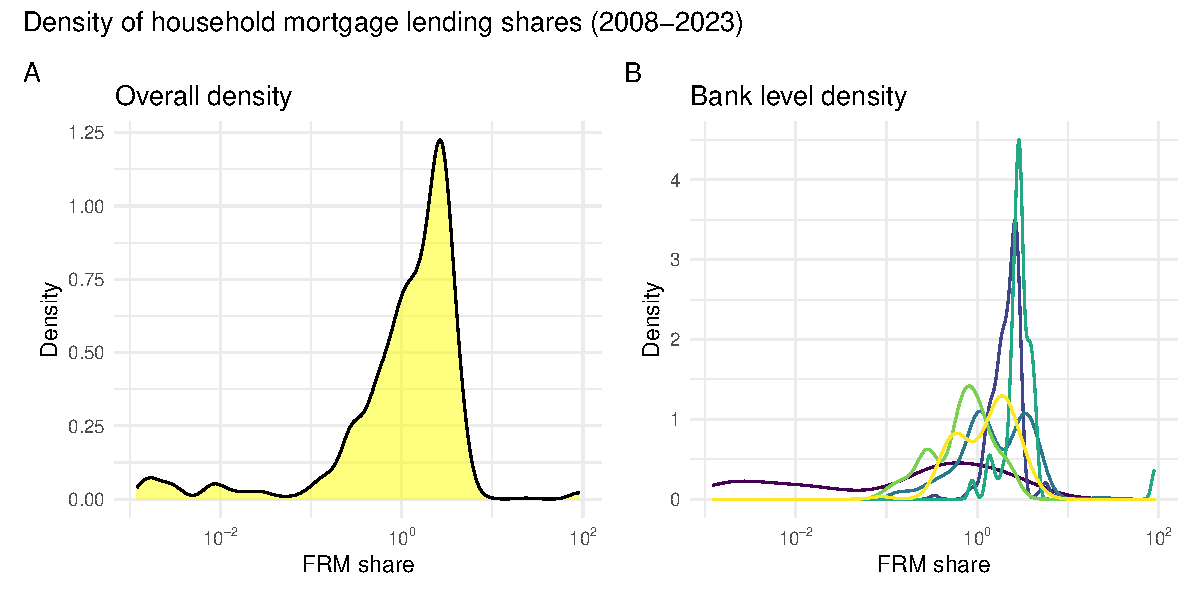
\includegraphics{mortgages_note_files/figure-pdf/fig-frm_density-1.pdf}

}

\caption{\label{fig-frm_density}Household FRM mortgage share density}

\end{figure}%

\begin{figure}[H]

\centering{

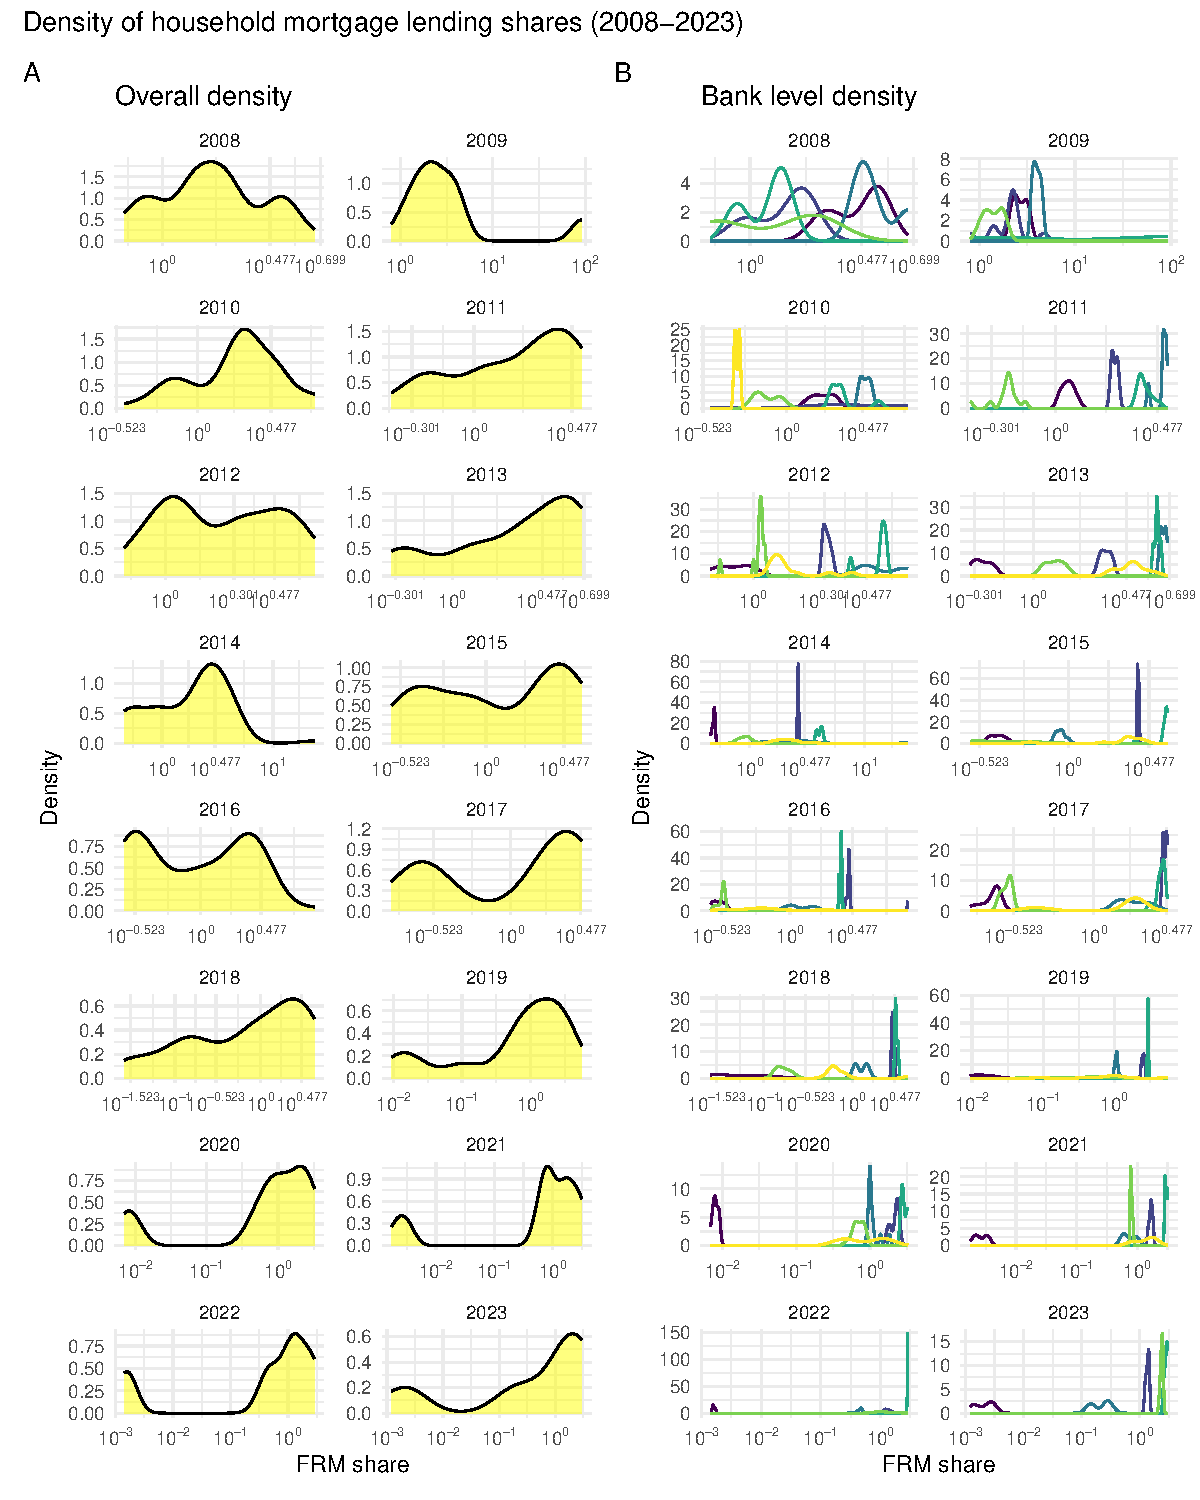
\includegraphics{mortgages_note_files/figure-pdf/fig-frm_density_year-1.pdf}

}

\caption{\label{fig-frm_density_year}Household FRM mortgage share
density by year}

\end{figure}%

\subsection{Distribution of household ARM mortgage
shares}\label{distribution-of-household-arm-mortgage-shares}

\begin{figure}[H]

\centering{

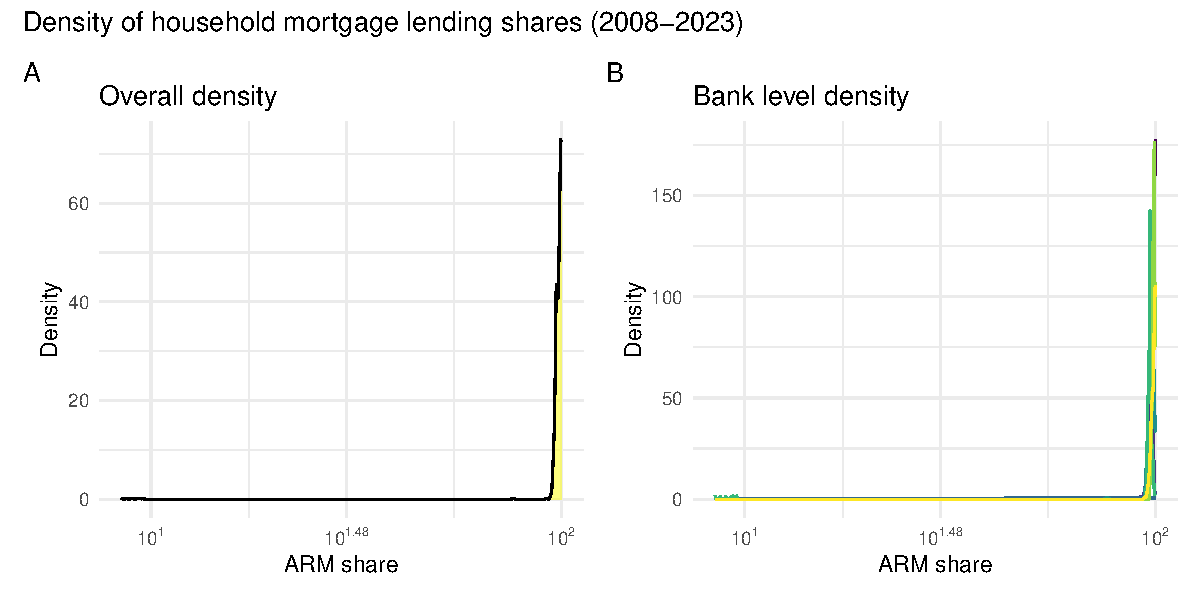
\includegraphics{mortgages_note_files/figure-pdf/fig-Arm_density-1.pdf}

}

\caption{\label{fig-Arm_density}Household ARM mortgage share density}

\end{figure}%

\begin{figure}[H]

\centering{

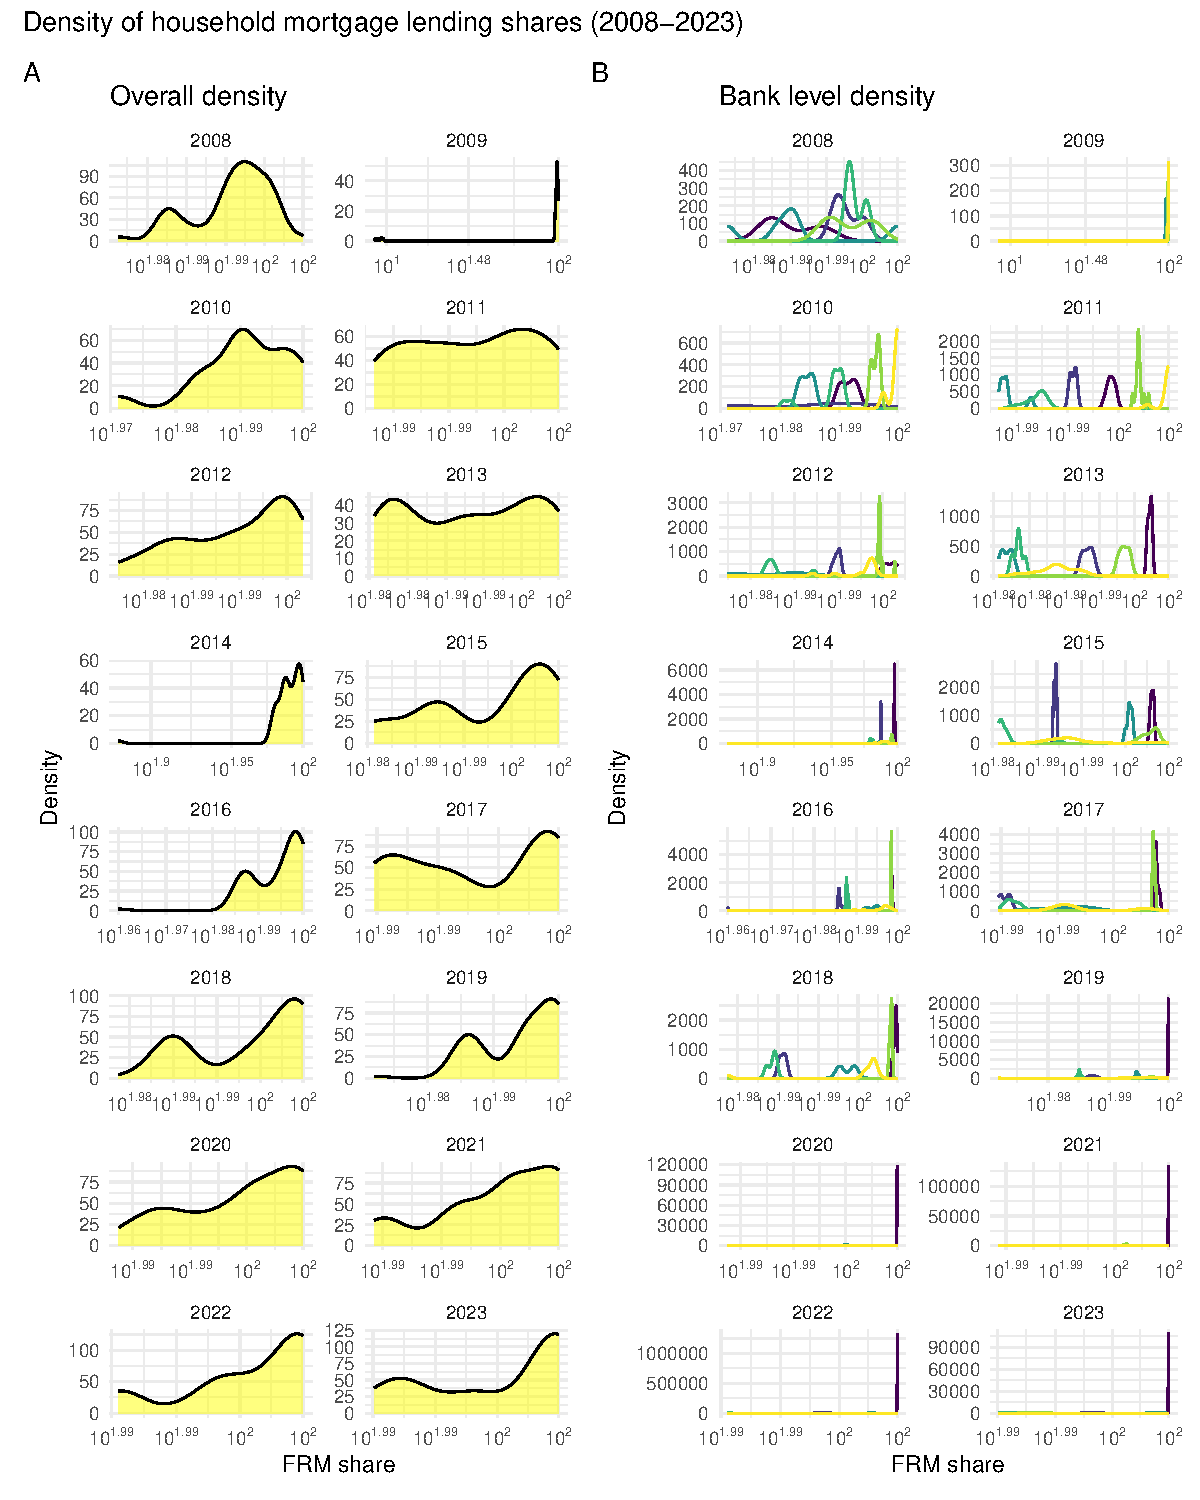
\includegraphics{mortgages_note_files/figure-pdf/fig-Arm_density_year-1.pdf}

}

\caption{\label{fig-Arm_density_year}Household ARM mortgage share
density by year}

\end{figure}%

\subsection{Binary outcomes of household mortgage
shares}\label{binary-outcomes-of-household-mortgage-shares}

\begin{figure}[H]

\centering{

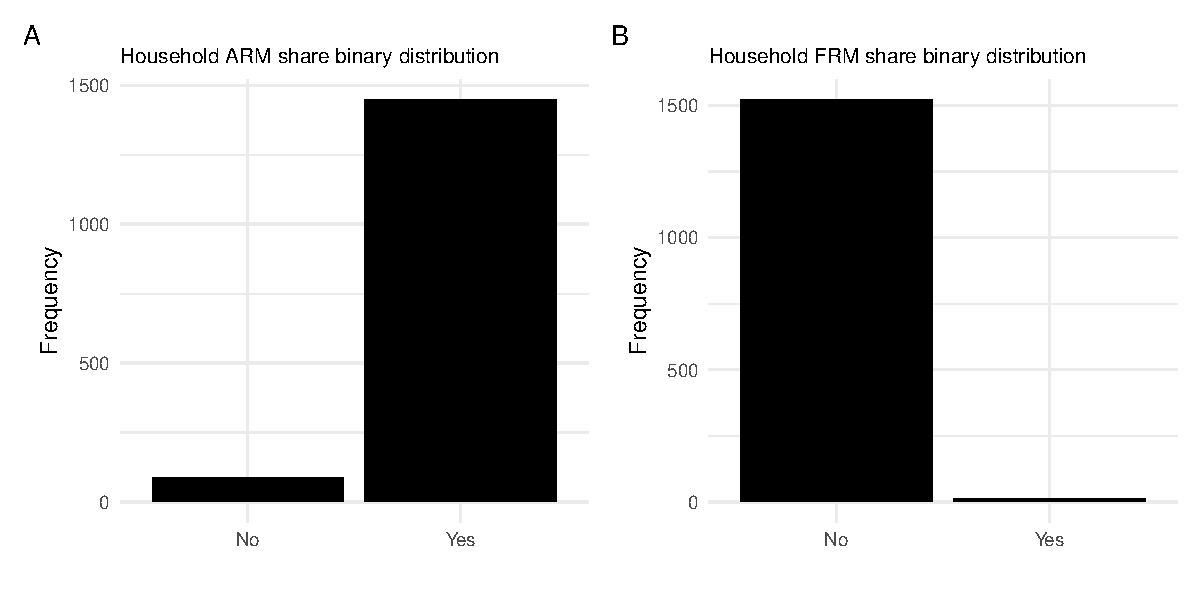
\includegraphics{mortgages_note_files/figure-pdf/fig-binary-1.pdf}

}

\caption{\label{fig-binary}Binary outcomes of household mortgage shares}

\end{figure}%




\end{document}
